%File: anonymous-submission-latex-2024.tex
\documentclass[letterpaper]{article} % DO NOT CHANGE THIS
% \usepackage[submission]{aaai24} % DO NOT CHANGE THIS
\usepackage{aaai24} % DO NOT CHANGE THIS
\usepackage{times} % DO NOT CHANGE THIS
\usepackage{helvet} % DO NOT CHANGE THIS
\usepackage{courier} % DO NOT CHANGE THIS
\usepackage[hyphens]{url} % DO NOT CHANGE THIS
\usepackage{graphicx} % DO NOT CHANGE THIS
\urlstyle{rm} % DO NOT CHANGE THIS
\def\UrlFont{\rm} % DO NOT CHANGE THIS
\usepackage{natbib} % DO NOT CHANGE THIS AND DO NOT ADD ANY OPTIONS TO IT
\usepackage{caption} % DO NOT CHANGE THIS AND DO NOT ADD ANY OPTIONS TO IT
\frenchspacing % DO NOT CHANGE THIS
\setlength{\pdfpagewidth}{8.5in} % DO NOT CHANGE THIS
\setlength{\pdfpageheight}{11in} % DO NOT CHANGE THIS
%

% These are recommended to typeset algorithms but not required. See the subsubsection on algorithms. Remove them if you don't have algorithms in your paper.

\usepackage{amsmath, amssymb}
\usepackage{algorithm}
\usepackage{algorithmic}
%
% These are are recommended to typeset listings but not required. See the subsubsection on listing. Remove this block if you don't have listings in your paper.
\usepackage{newfloat}
\usepackage{listings}
\DeclareCaptionStyle{ruled}{labelfont=normalfont, labelsep=colon, strut=off} % DO NOT CHANGE THIS
\lstset{%
	basicstyle={\footnotesize\ttfamily}, % footnotesize acceptable for monospace
	numbers=left, numberstyle=\footnotesize, xleftmargin=2em, % show line numbers, remove this entire line if you don't want the numbers.
	aboveskip=0pt, belowskip=0pt, %
	showstringspaces=false, tabsize=2, breaklines=true}
\floatstyle{ruled}
\newfloat{listing}{tb}{lst}{}
\floatname{listing}{Listing}
%
% Keep the \pdfinfo as shown here. There's no need
% for you to add the /Title and /Author tags.
\pdfinfo{
/TemplateVersion (2024.1)
}

\usepackage{amsfonts, array, makecell, bm, multirow, soul, cancel, xcolor, textcomp, cite, lineno}


\def \eg {\emph{e.g.}}
\def \ie {\emph{i.e.}}
\def \etal {\emph{et al. }}

\newcommand\red[1]{\textcolor{red}{#1}}
\newcommand\blue[1]{\textcolor{blue}{#1}}
\newcommand\purple[1]{\textcolor{purple}{#1}}
\newcommand\rbb[1]{\textcolor{red}{\{RB: #1\}}}
\newcommand\rjf[1]{\textcolor{red}{\{RJF: #1\}}}
\newcommand\zjl[1]{\textcolor{blue}{\{ZJL: #1\}}}
\newcommand\yxy[1]{\textcolor{blue}{\{YXY: #1\}}}
\newcommand\hwt[1]{\textcolor{purple}{\{HWT: #1\}}}
\newcommand\qz[1]{\textcolor{blue}{\{QZ: #1\}}}


% DISALLOWED PACKAGES
% \usepackage{authblk} -- This package is specifically forbidden
% \usepackage{balance} -- This package is specifically forbidden
% \usepackage{color (if used in text)
% \usepackage{CJK} -- This package is specifically forbidden
% \usepackage{float} -- This package is specifically forbidden
% \usepackage{flushend} -- This package is specifically forbidden
% \usepackage{fontenc} -- This package is specifically forbidden
% \usepackage{fullpage} -- This package is specifically forbidden
% \usepackage{geometry} -- This package is specifically forbidden
% \usepackage{grffile} -- This package is specifically forbidden
% \usepackage{hyperref} -- This package is specifically forbidden
% \usepackage{navigator} -- This package is specifically forbidden
% (or any other package that embeds links such as navigator or hyperref)
% \indentfirst} -- This package is specifically forbidden
% \layout} -- This package is specifically forbidden
% \multicol} -- This package is specifically forbidden
% \nameref} -- This package is specifically forbidden
% \usepackage{savetrees} -- This package is specifically forbidden
% \usepackage{setspace} -- This package is specifically forbidden
% \usepackage{stfloats} -- This package is specifically forbidden
% \usepackage{tabu} -- This package is specifically forbidden
% \usepackage{titlesec} -- This package is specifically forbidden
% \usepackage{tocbibind} -- This package is specifically forbidden
% \usepackage{ulem} -- This package is specifically forbidden
% \usepackage{wrapfig} -- This package is specifically forbidden
% DISALLOWED COMMANDS
% \nocopyright -- Your paper will not be published if you use this command
% \addtolength -- This command may not be used
% \balance -- This command may not be used
% \baselinestretch -- Your paper will not be published if you use this command
% \clearpage -- No page breaks of any kind may be used for the final version of your paper
% \columnsep -- This command may not be used
% \newpage -- No page breaks of any kind may be used for the final version of your paper
% \pagebreak -- No page breaks of any kind may be used for the final version of your paperr
% \pagestyle -- This command may not be used
% \tiny -- This is not an acceptable font size.
% \vspace{- -- No negative value may be used in proximity of a caption, figure, table, section, subsection, subsubsection, or reference
% \vskip{- -- No negative value may be used to alter spacing above or below a caption, figure, table, section, subsection, subsubsection, or reference

\setcounter{secnumdepth}{0} %May be changed to 1 or 2 if section numbers are desired.

% The file aaai24.sty is the style file for AAAI Press
% proceedings, working notes, and technical reports.
%

% Title

% Your title must be in mixed case, not sentence case.
% That means all verbs (including short verbs like be, is, using, and go), 
% nouns, adverbs, adjectives should be capitalized, including both words in hyphenated terms, while
% articles, conjunctions, and prepositions are lower case unless they
% directly follow a colon or long dash
\title{Scale Optimization Using Evolutionary Reinforcement Learning for Object Detection on Drone Imagery}
\author{
  %Authors
  % All authors must be in the same font size and format.
  $^\dagger$Jialu Zhang\textsuperscript{\rm 1,3}, 
  $^\dagger$Xiaoying Yang\textsuperscript{\rm 1}, 
  Wentao He\textsuperscript{\rm 1}, 
  \thanks{Corresponding author. $^\dagger$Equal contribution.}Jianfeng Ren\textsuperscript{\rm 1,2},
  Qian Zhang\textsuperscript{\rm 1,2},
  Yitian Zhao\textsuperscript{\rm 3},
  Ruibin Bai\textsuperscript{\rm 1,2},
  Xiangjian He\textsuperscript{\rm 1,2},
  Jiang Liu\textsuperscript{\rm 3,4}
}
\affiliations{
  %Afiliations
  \textsuperscript{\rm 1}The Digital Port Technologies Lab, School of Computer Science, University of Nottingham Ningbo China\\
  \textsuperscript{\rm 2}Nottingham Ningbo China Beacons of Excellence Research and Innovation Institute, University of Nottingham Ningbo China\\
  \textsuperscript{\rm 3}Cixi Institute of Biomedical Engineering, Chinese Academy of Sciences\\
  \textsuperscript{\rm 4}Department of Computer Science and Engineering, Southern University of Science and Technology\\
  \{sgxjz1,scxxy1,scxwh1,jianfeng.ren,qian.zhang, ruibin.bai,sean.he\}@nottingham.edu.cn, yitian.zhao@nimte.ac.cn, liuj@sustech.edu.cn}


% REMOVE THIS: bibentry
% This is only needed to show inline citations in the guidelines document. You should not need it and can safely delete it.
\usepackage{bibentry}
% END REMOVE bibentry


\begin{document}

\maketitle

\begin{abstract}
Object detection in aerial imagery presents a significant challenge due to large scale variations among objects. This paper proposes an evolutionary reinforcement learning agent, integrated within a coarse-to-fine object detection framework, to optimize the scale for more effective detection of objects in such images. 
% \blue{\{Confusing. Both missing GT issue and find optimal scale task are for patches, but this sentence seems for objects, which suppose have GT annotations.\}}. % following a coarse-to-fine pipeline. %in which %designing image cropping strategies, i.e., generating patches 
Specifically, a set of patches potentially containing objects are first generated. 
% by a YOLOX variant, expanded to include the background context, and merged to form the cluster regions. 
%YOLOX with an extra set of feature maps for detecting ultra-small objects. 
%To address the challenges of lacking ground-truth optimal scale for each patch, the scale selection is formulated as a Markov decision process and an evolutionary reinforcement learning agent is designed to determine the optimal scale. In this scale, we can better capture the fine-grained details of the object by enlarging the scale, while minimizing the artifacts caused by excessive scaling. 
A set of rewards measuring the localization accuracy, the accuracy of predicted labels, and the scale consistency among nearby patches are designed in the agent to guide the scale optimization. The proposed scale-consistency reward ensures similar scales for neighboring objects of the same category. 
Furthermore, a spatial-semantic attention mechanism is designed to exploit the spatial semantic relations between patches. 
% for better scale prediction. 
The agent employs the proximal policy optimization strategy in conjunction with the evolutionary strategy, effectively utilizing both the current patch status and historical experience embedded in the agent.  
%trains the network more effectively. 
The proposed model is compared with state-of-the-art methods on two benchmark datasets for object detection on drone imagery. It significantly outperforms all the compared methods. %Code is available at https://github.com/UNNC-CV/EvOD/.
\end{abstract}

\section{Introduction}
\label{sec: intro}

%\rjf{Background}
%Because of its good mobility and stability, 
Unmanned Aerial Vehicles have been widely used in various applications, \eg, surveillance~\cite{Yun_2022_surveillance}, autonomous detection~\cite{REN_2017_UAVDetection, REN_2021_UAVDetection}, fleet navigation~\cite{Alami_2023_FleetNavigation} and agriculture~\cite{Tokekar_2016_agriculture}. %To enable the vision capability of drones, 
Object detection from drone-captured images has attracted research attention recently~\cite{Xi_2021_SeanHE, Yue_2020_SeanHe, Bouguettaya_2022_review}. %Benefiting from the development of deep learning techniques, 
Although object detection on natural images has progressed significantly~\cite{Ge_2021_YOLOX}, detecting objects in aerial images remains challenging, mainly stemming from small scales and extreme scale variations~\cite{Deng_2021_GLSAN, Xu_2022_AdaZoom}. 

\begin{figure}[t]
	\centering
	\centerline{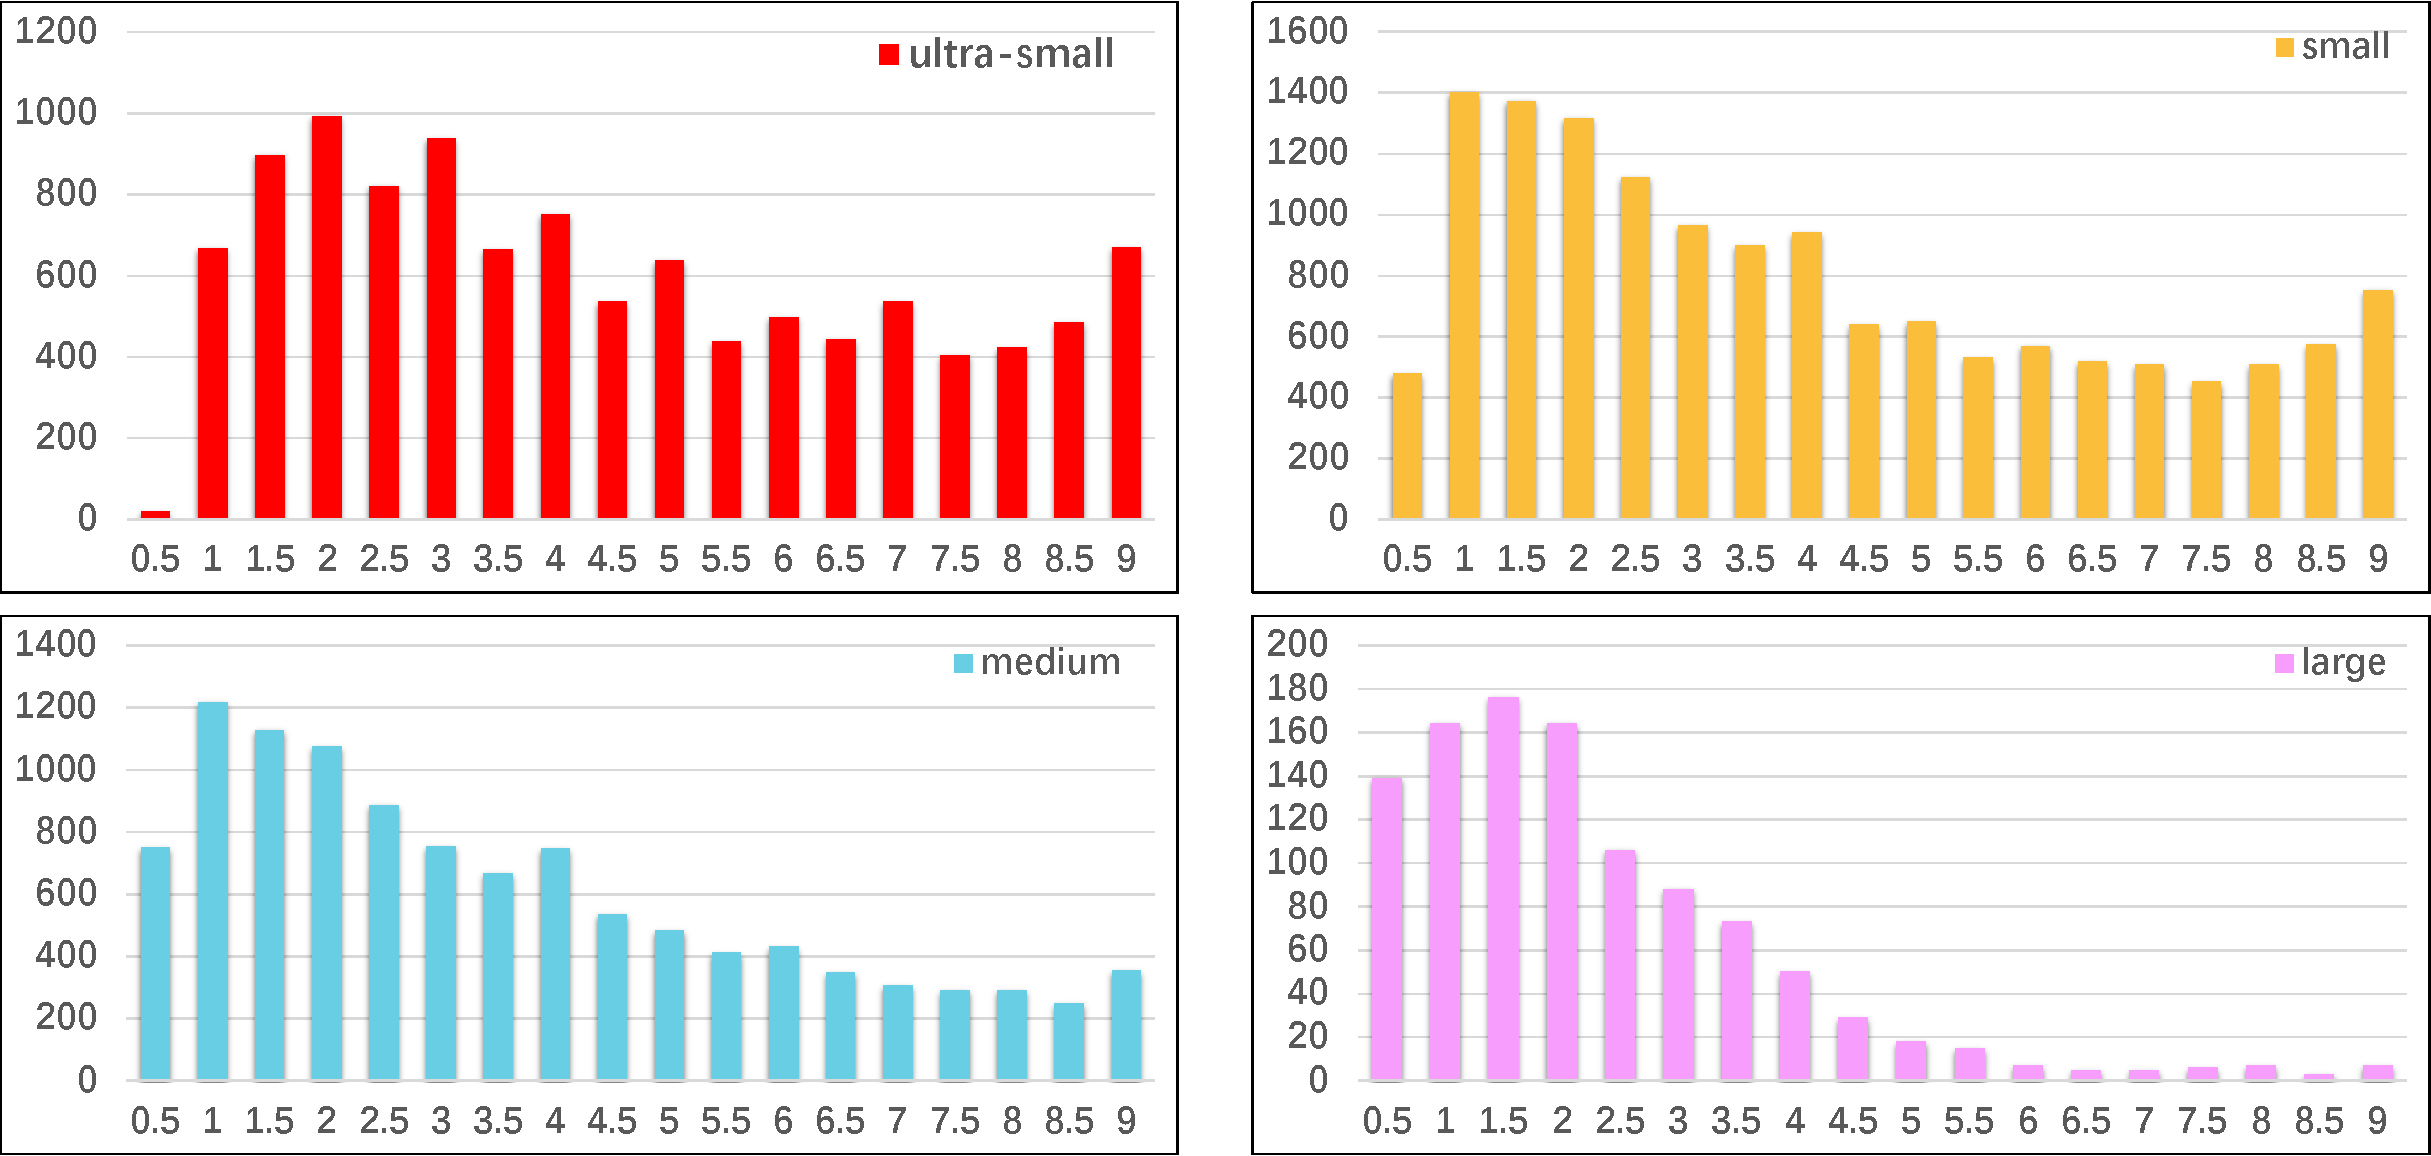
\includegraphics[width= 1\columnwidth]{./images/Intro1.pdf}}
	\caption{%(a) An example of the VisDrone dataset, where objects are annotated with different colours according to the ground-truth annotations. Red, orange, light blue, pink, and dark blue represent extra-small, small, medium, large, and extra-large objects, respectively. (b)-(e) 
 The number of objects (\textit{y-axis}) that are optimally detected using the scaling factor (\textit{x-axis}) for ultra-small, small, medium and large objects, respectively on the VisDrone dataset. \textit{The optimal scales are significantly different for different objects.}% \qz{The figure shows the optimal detection of objects based on their size using different scaling factors on the VisDrone dataset. The \textit{y-axis} represents the number of objects detected, while the \textit{x-axis} represents the scaling factor. The optimal scales for ultra-small, small, medium, and large objects are significantly different.}} %Although in most cases objects are better detected by scaling up, in the cases of scaling factor of 0.5, the objects are better detected by scaling down. 
 % \rjf{ultra-small}. 
 % \rjf{1. Remove Image (a). 2. Enlarge the very small text in (b)-(e). Requirement: The given text should be large enough to visually recognize it.}
 }
	\label{fig: intro}
\end{figure}



%\rjf{Categorization, review}
%Aerial scenes are typically dominated by small objects. Continuous downsampling operations on large scene images often lead to the loss of semantic and spatial information of small objects, so 

%The objects 
Objects in aerial scenes often have large-scale variations, \eg, %distant objects may only occupy a few pixels while nearby objects may occupy hundred thousands of pixels. 
distant objects occupy few pixels while nearby objects occupy thousands. %Such a large scale change makes it difficult to detect objects in aerial scenes. Early methods %simply treated UAV detection as a case of the small object detection problem, 
%Early methods often adapt general object detection methods for drone imagery, and concentrate on enhancing small object detection~\cite{Cheng_2019_Learning, Bai_2018_SODMTGAN}. 
%Cheng \etal introduced novel objective functions to enrich the representation power of object detection models for small objects~\cite{Cheng_2019_Learning}. 
%Li \etal and Bai \etal utilized generative adversarial networks to obtain the fine-grained feature representations for small blurred objects~\cite{Li_2017_Perceptual, Bai_2018_SODMTGAN}. % Li \emph{et, al.} design an up-sampling module to transform the original poor features of small objects into super-resolved and high-discriminative ones~\cite{Li_2017_Perceptual}.~\cite{Bai_2018_SODMTGAN} introduce generative adversarial network to obtain fine-grained feature representations for small blurred images. 
% Deep convolutional layers provide powerful semantics for detecting large objects, but they perform poorly in detecting small objects~\cite{XIAO_2023_TinyReview}. Taking advantages of the high-resolution feature maps of shallow layers, \citet{Bouguettaya_2022_review} designed a shallow network to enhance small vehicle detection on aerial imagery, while \citet{Sommer_2017_Fast} leveraged feature maps from shallow layers to boost the detector performance. %The feature pyramid network (FPN) is often adopted to combine low-level features in shallow layers and high-level features in deep layers for multi-scale vehicle detection~\cite{Gu_2018_FPNVehicle, Wang_2019_VehicleFPN, Zhou_2019_SAICFPN}. %~\cite{Sommer_2018_Deconvolutional} upsamples the low-dimensional feature maps of deeper layers through deconvolutional layers, and combines them with shallower layer feature maps to detect small vehicles from aerial images. 
%For object detection in aerial scenes, the small objects are most difficult to detect~\cite{Bouguettaya_2022_review}. 
To tackle the challenges of detecting small objects and/or objects of different sizes, a common strategy is to divide an image into patches, scale the patches containing small objects to a fixed size~\cite{Deng_2021_GLSAN, Xu_2022_AdaZoom} or using one or more fixed scaling factors~\cite{Huang_2022_UFPMP}, and then feed them into an object detector. 
%With a view to better detecting small objects, it is crucial to enlarge the focused area. Existing solutions introduce some strategies to achieve that, such as scaling all patches to a fixed size, scaling all patches with one or more fixed scale factors, etc. However, the optimal scale of each patch has not been fully exploited. 
But the patch scalability is inherently limited %, requiring thoughtful consideration of scaling ratios. This constraint arises 
%not only due to the computational resource limitations but also the %propensity of up-sampling to induce image blur and compromise the preservation of fine details. 
due to the potential image artifacts caused by excessive scaling. 
%can render objects indistinguishable, regardless of their size. \rjf{What does it mean?} %Overscaling can result in objects being indistinguishable. 
Moreover, patches may encompass objects of different sizes. While enlarging a patch improves detecting small objects, it also enlarges large objects, potentially impeding their recognition. As shown in Fig.~\ref{fig: intro}, the optimal scales for different objects vary significantly. It is hence crucial to determine the optimal scale of each patch. 


However, there lacks ground-truth annotations for the optimal scales. To tackle this problem, an EVOlutionary Reinforcement Learning (EVORL) agent is designed to determine the most suitable scale for each patch, with the guidance of a carefully designed reward function. This function assesses the image patch by considering the localization accuracy, the accuracy of predicted labels, and the scale consistency among nearby patches. The first two are directly related to the performance of object detection while the last one regularizes the optimized scales. This scale consistency stems from the inherent characteristics of drone imagery, where nearby objects of the same category tend to exhibit a similar scale. By rewarding the scale consistency, the agent is able to eliminate outliers influenced by incidental factors, thereby contributing to an improved detection performance. 


Simultaneously optimizing the three rewards may result in potential conflicts, complicate the training convergence, and limit the performance. To mitigate this issue, an evolutionary strategy is integrated into the reinforcement learning framework. Specifically, the optimal scales of all patches during training are combined with sampled historical solutions to form an initial population. The proposed evolutionary algorithm refines the optimal scale determined by the current patch status by evolving the solutions using mutation and crossover, taking into account of the scale consistency among nearby patches. By incorporating both the current patch status and past experience stored in the agent's population, the proposed EVORL effectively determines the optimal scale for precise object detection.


To further boost the detection performance, a spatial-semantic attention is developed. Intuitively, spatially close objects could not only exhibit the scale consistency, but also provide the spatial-semantic attention to mutually enhance the patch features~\cite{he2023hierarchical,Zhang_2023_Spatial}. %Specifically, the proposed method models the spatial attention by measuring the distance between nearby objects, and models the semantic attention by measuring the pairwise appearance correlation between objects, and these two attentions are aggregated to obtain the spatial-semantic attention. 
Specifically, the proposed method models the spatial and semantic attention by measuring the distances and the pairwise appearance correlations between adjacent objects, respectively, and aggregates these two to obtain the spatial-semantic attention. The proposed spatial-semantic attention could effectively model the spatial and semantic dependencies between objects, enhance the patch features and finally help to better detect objects at a most appropriate scale. 


The proposed method follows a coarse-to-fine object detection pipeline~\cite{Bouguettaya_2022_review}. Specifically, a YOLOX~\cite{Ge_2021_YOLOX} variant is utilized to coarsely generate regions of interests. These regions are expanded to include the background context and merged to form cluster regions as in~\cite{Huang_2022_UFPMP}. A feature extractor with the proposed spatial-semantic attention is designed to visually perceive the regions. The perceived information is transmitted to the proposed EVORL agent to determine the optimal scale for each region, with the guidance of the three carefully designed rewards. Finally, the scaled regions are fed back to the detector for fine detection. 


Our contributions can be summarized as follows. 1) The proposed EVORL agent is seamlessly integrated into a coarse-to-fine object detection framework, and makes use of both the current image patch and the past experience embedded in the agent to determine the optimal scale to accurately detect objects. 2) The designed reward function well addresses the challenges of lacking ground-truth labels for optimal scales, and provides supervision signals to train the agent. The proposed scale-consistency reward considers the scales of both the current object and nearby objects, to eradicate outliers and enhance the detection performance. 3) The proposed spatial-semantic attention exploits the spatial and semantic relations between nearby patches, to enhance the discriminant power of patch features. 4) The proposed method significantly outperforms state-of-the-art methods for object detection, improving the previous best average precision from 24.6\% to 28.0\% on the UAVDT dataset, and from 40.3\% to 42.2\% on the VisDrone dataset. 


\section{Related Work}
\label{sec: related-work}
\subsection{Object Detection on Drone Imagery}
In aerial images, there are a large number of small objects, \eg, 26.5\% of objects in the VisDrone dataset~\cite{Zhu_2022_VisDrone} occupying fewer than $16^2$ pixels. Researchers have strove to improve small object detection on aerial imagery by adapting general object detectors on natural images. For example, \citet{Cheng_2019_Learning} designed novel objective functions for small object detection without altering existing network architectures. \citet{Li_2017_Perceptual} developed a super-resolution technique to enlarge the image for better detecting small objects. \citet{Bai_2018_SODMTGAN} utilized a generative adversarial network to obtain fine-grained features for small blurred objects. Some researchers utilized the shallow layers of deep neural networks to alleviate the problems of low resolution and detail loss caused by down-sampling operations~\cite{Bouguettaya_2022_review}, \eg, \citet{Sommer_2017_Fast} used high-resolution feature maps from earlier layers to enhance detection performance. 

Some researchers tackled the challenges of large scale variations. \citet{Wang_2019_Spatial} introduced a Receptive Field Expansion Block and a Spatial-Refinement Module to capture context information and refine solutions using multi-scale pyramid features. \citet{Zhang_2019_Scale} developed a scale-adaptive proposal network, which consists of multi-scale region proposal networks and multi-layer feature fusion to better detect objects of different scales. The feature pyramid network is often adopted to combine low-level features from shallow layers with high-level features from deep layers for multi-scale object detection~\cite{Zhou_2019_SAICFPN}. 


The coarse-to-fine pipeline is often utilized for detecting objects in aerial images through extracting regions of interests using a coarse detector, scaling the image patches, and then detecting objects within them~\cite{Bouguettaya_2022_review}. \citet{Unel_2019_TilingSOD} uniformly divided the high-resolution image into patches of a fixed size, and detected objects from patches. \citet{Yang_2019_Clustered} designed a network to crop regions of dense objects and a scale estimation network to resize the crops. \citet{Xu_2022_AdaZoom} developed a self-adaptive region selection algorithm to focus on the dense regions, and leveraged super-resolution to enlarge the focused regions to a fixed size before fine-grained detection. \citet{Huang_2022_UFPMP} first equalized the scales of all generated patches, and then fed them into a unified mosaic for inference. 

Although scaling is critical to object detection, existing solutions often scale the patches to a fixed size~\cite{Xu_2022_AdaZoom} or using fixed scaling factors~\cite{Huang_2022_UFPMP}. Optimal scaling has not been fully exploited. 

\subsection{General Object Detection}
General object detectors are often adapted for drone imagery~\cite{Cai_2018_Cascade}. % We hence briefly review these methods here. 
Depending on the way of feature extraction, object detectors can be broadly divided into traditional methods and deep learning methods. Traditional methods often utilize handcrafted features such as local binary patterns~\cite{Ren_2015_LBPVisualRecognition}, scale-invariant key-points~\cite{Lowe_2004_SIFT} and histograms of oriented gradients~\cite{Dalal_2005_HOG}. % for object detection. %These features are often concatenated \rjf{reference}\blue{? Why is the reference required here but not after `aggregation'? } or aggregated by using feature pooling encoders such as Spatial Pyramid Matching models~\cite{2006_Lazebnik_Beyond}. 
These handcrafted features are often task-specific, and ineffective in dealing with complex real-world problems~\cite{Bouguettaya_2022_review}.

\begin{figure*}[!tb]
	\centering
	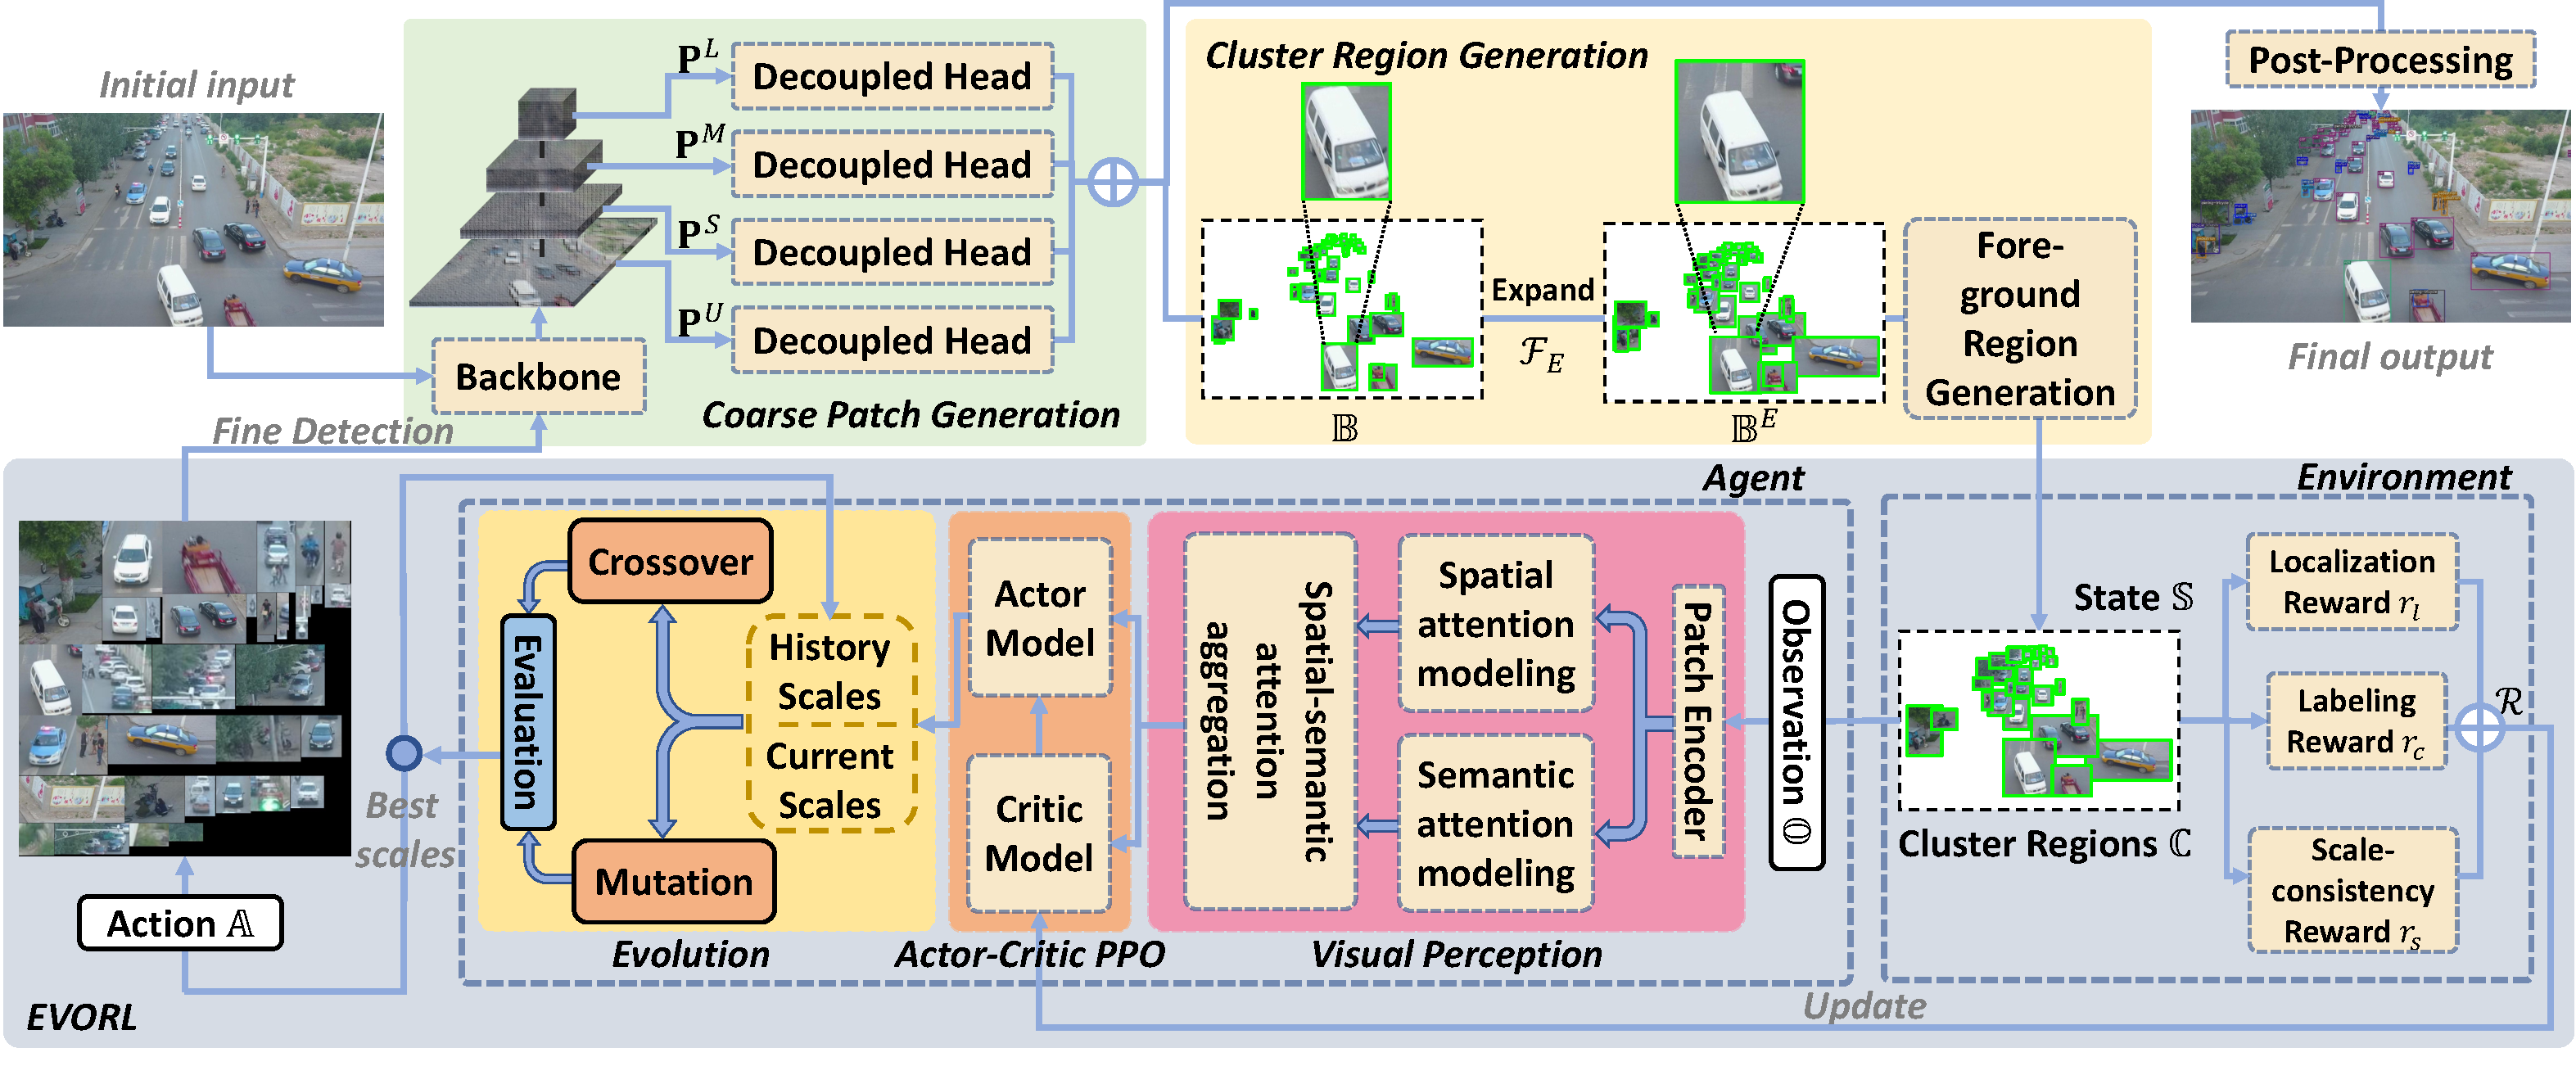
\includegraphics[width= \linewidth]{images/structure2.pdf}
	\caption{Overview of the proposed model.
 A YOLOX variant is first utilized to generate regions of interests. The regions are expanded to include the background context and merged to form cluster regions. An evolutionary reinforcement learning (EVORL) agent with three rewards %for the localization accuracy, the accuracy of predicted labels and the scale consistency 
 is designed to determine the optimal scale for each patch. The spatial-semantic attention is designed to boost the patch features. After determining the optimal scales through the proposed EVORL, the regions are scaled and consolidated into a mosaic image, and passed back to the detector for fine detection. %Finally, a set of post-processing techniques including non-maximal suppression are utilized to generate the detection results. 
 %It consists of three main stages: coarse patch generation, adaptive scale selection for the generated patches, and detailed detection. Within the framework, detectors are adapted from YOLOX~\cite{Ge_2021_YOLOX}, with an addition of a small-scale feature map for more details. The process begins with producing a set of coarsely detected patches, enabled by a coarse detector and in alignment with the foreground region generation algorithm as proposed in~\cite{Huang_2022_UFPMP}. Subsequently, the determination of the optimal scale for these patches is formulated as a Markov Decision Problem (MDP) and handled with Deep Reinforcement Learning (DRL) techniques in an adaptive manner. These rescaled patches are then consolidated into a mosaic image, serving as the input for the final detailed detection stage.
 %\rjf{1. Feature extractor: is it a backbone network or what?} \blue{a backbone network used to generate the feature pyramid. According to the original paper of YOLOX, it should be CSPDarkNet (proposed in v4, devised in scaledv4 \& v5 (v5 is code only, no paper). The output of the backbone, FPN, is enhanced by PAN operation (v4). Scaled-v4 improved this with 'CSP-ize the PAN'. The additional small-scale layer introduced in this paper is at this part (the output of backbone contains 5 layers, while only 3 are used in v4, scaledV4, v5 and X. We use four of them).)}
 %\rjf{More details are needed for the key building blocks. 1. YOLOX could be simplified or made smaller. 2. More details for Cluster Region Generation. 3. Much more details for EVO-DRL. Put more emphasis on this.}
 %\rjf{1. Building block names: spatial attention extraction, semantic attention extraction, spatial-semantic attention aggregation. Name put into building blocks. 2. The attention between nearby objects can't be seen from the figure. 3. The drawing for these three blocks seems to be too simple. It is significantly different from our TIP paper. There are two solutions: a). Further simplify it into three building blocks with names only, e.g. Two parallel building blocks for spatial attention extraction and semantic attention extraction, followed by spatial-semantic attention aggregation. b) Try to use the similar drawing as in TIP. 4. Enlarge the building for `Policy Net'. Change the name to ` Proximal Policy Optimization Network'?}
 } 
	\label{fig: structure}
\end{figure*}

%Deep learning techniques tackle this issue through extracting features automatically in a learned approach~\cite{Liu_2020_ODSurvey, He_2016_Deep, Xie_2017_Aggregated}, where convolutional networks are used as network backbones in object detection frameworks. 
Numerous deep learning object detectors have been developed recently~\cite{Ren_2017_Faster, Ge_2021_YOLOX}, %which 
and they demonstrate superior performance thanks to the discriminative deep learning features. 
%Based on these powerful backbone networks, many object recognition frameworks are derived. According to the detection pipeline, 
These models could be further categorized into two types: 1) Two-stage detectors, in which regions of interests are first extracted using a region proposal network, and objects are recognized within them. %, \eg, 
Representative models include %regions with CNN features (R-CNN)~\cite{Girshick_2014_Rich}, Fast R-CNN~\cite{Girshick_2015_Fast}, Faster R-CNN~\cite{Ren_2017_Faster}, Mask R-CNN~\cite{He_2017_Mask} and Cascade R-CNN~\cite{Cai_2018_Cascade}. 
Regions with CNN features (R-CNN)~\cite{Girshick_2014_Rich}, Faster R-CNN~\cite{Ren_2017_Faster}, and Mask R-CNN~\cite{He_2017_Mask}. 2) One-stage detectors, which integrate the proposal generation and object detection into one stage. YOLO-series (You Only Look Once)~\cite{Redmon_2016_You, Redmon_2017_YOLO9000, Ge_2021_YOLOX}, %Single Shot MultiBox Detector (SSD)~\cite{Liu_2016_SSD} and RetinaNet~\cite{Lin_2020_Focal} are the representative solutions. 
RetinaNet~\cite{Lin_2020_Focal} and EfficientDet~\cite{Tan_2020_EfficientDet} are the leading solutions.


General object detectors perform well on natural images, % \eg, the MS COCO dataset~\cite{Lin_2014_COCO} and the PASCAL VOC dataset~\cite{Everingham_2010_PASCAL}. 
but not on aerial images. Aerial images often have higher image resolution but contain much more objects of various sizes, which imposes great challenges for detecting them. %(\emph{e.g.} the resolution of each image is around 640×480 in MS COCO~\cite{Lin_2014_COCO} and 500×400 in PASCAL VOC~\cite{Everingham_2010_PASCAL}, while 2, 000×1, 500 in VisDrone~\cite{Zhu_2022_VisDrone} and 1, 024×540 in UAVDT~\cite{Du_2018_UAVDT}). In addition, Detecting small objects in high-resolution images, especially drone images, has received increasing research attention.



\section{Proposed Method}
\label{sec: methodology}

% \subsection{Motivations of Proposed Method}
% % \rjf{Move some of the previous discussions here.}
% \rjf{1. Why optimize scale, small scales and Large scale variations, scaling key step in many methods.
% 2. Why DRL, no ground-truth labels.
% 3. Why three rewards. 
% 4. Why Spatial-semantic attention. 
% 5. Why EVO-DRL}

% The coarse-to-fine pipeline is often utilized to better detect objects on drone imagery, \ie, regions of interest are first extracted using a coarse detector and then subject to finer detection~\cite{Ge_2022_ZoomAndReasoning, Yang_2019_Clustered, Li_2020_Density_Workshops, Huang_2022_UFPMP, Xu_2022_AdaZoom}.


% Compared to natural images, object detection in aerial images presents unique challenges due to small object sizes, large scale variations, among others. Previous solutions address these challenges by devising a coarse-to-fine pipeline, where regions are first detected coarsely and then forwarded to a finer detector for detailed analysis. One crucial but often overlooked step in this pipeline is re-scaling these coarsely detected regions. Existing approaches typically employ fixed sizes, potentially leading to miss detected objects and inaccurate bounding box predictions due to inappropriate scales. Thus, we propose a novel scale-selection algorithm that leverages deep reinforcement learning techniques, aiming to adaptively identify the optimal scale for each coarsely detected region.

% Notably, objects captured in drone imagery of the same category and spatial proximity tend to share similar scales. With this observation, we introduce a constraint aiming to determine the optimal scale for each patch thereby enhancing detection accuracy. Unlike existing solutions that measure their results based solely on detection accuracy, the proposed method considers not only the detection accuracy but also the scale-consistency across different patches. Motivated by these considerations, we present a novel object detection method for drone imagery employing deep reinforcement learning techniques. To provide feedback to the deep reinforcement learning network, a spatial attention reward is devised, taking into account both detection accuracy and scale-consistency. This not only guides the optimization of the network but also addresses the challenge of unlabeled training.


\subsection{Overview of Proposed Method}
\label{sec: overallFramework}

% \rjf{Please draft the block diagram first. The proposed method is not clear yet.} 



% \rjf{1. Why optimize scale, small scales and Large scale variations, scaling key step in many methods.
% 2. Why DRL, no ground-truth labels.}

% The detection of small objects and objects with large-scale changes in aerial images often poses great challenges. %Existing methods often first derive the image patches potentially containing objects, scale the patches and detect objects within them~\cite{Yang_2019_Clustered, Huang_2022_UFPMP, Xu_2022_AdaZoom}. Indeed, scaling up small objects \rjf{references} or scaling objects to a fixed size \rjf{references} help object detection. But the optimal scale of each patch has not been fully exploited in literature. %\blue{\{confusing with aforementioned sentence. What's the difference between scaling patches work and scaling objects approaches?\}}. 
% One potential reason is the lack of ground-truth labels for the optimal scale at which the object is best detected. 
%The optimal scale of each patch is crucial to the object detection performance on drone imagery. 
To tackle the challenges of determining the optimal scales, 
an evolutionary reinforcement learning agent is proposed. The agent is integrated into a coarse-to-fine object detection framework. The proposed framework mainly consists of three modules, as shown in Fig.~\ref{fig: structure}. 
1) \textbf{Coarse Patch Generation}. %, where a variant of YOLOX~\cite{Ge_2021_YOLOX} is utilized to derive the regions of interests. Specifically, 
CSPDarkNet~\cite{Wang_2021_ScaledYOLOv4} is utilized as the backbone to generate the feature pyramid. %$\mathbb{P}$. 
In addition to the small, medium and large feature maps $\bm{\mathsf{P}}^S,\bm{\mathsf{P}}^M,\bm{\mathsf{P}}^L$ used in YOLOX~\cite{Ge_2021_YOLOX}, an ultra-small feature map $\bm{\mathsf{P}}^{U}$ is added, which contains low-level fine details for better detecting small objects. 
These features are then fed into the YOLOX decoupled heads to generate regions of interests $\mathbb{B}$. % as $\mathbb{B} = \mathcal{F}_r(\bm{\mathsf{P}}^{U}, \bm{\mathsf{P}}^{S}, \bm{\mathsf{P}}^{M}, \bm{\mathsf{P}}^{L})$, where $\mathcal{F}_r$ represents the function for generating the regions of interest (ROI) sets $\mathbb{B}$ from feature maps. 
%Specifically, a backbone network, CSPDarkNet~\cite{Wang_2021_ScaledYOLOv4}, is utilized to generate the feature pyramid. In addition to the three output layers for small, medium and large feature maps used in YOLOX \rjf{reference}, a layer for ultra-small feature map is added to better detect small objects. These features are then fed into the YOLOX decoupled heads to generate regions that potentially contain objects. 
%According to the original paper of YOLOX, it should be CSPDarkNet (proposed in v4, devised in scaledv4 \& v5 (v5 is code only, no paper). The output of the backbone, FPN, is enhanced by PAN operation (v4). Scaled-v4 improved this with 'CSP-ize the PAN'. The additional small-scale layer introduced in this paper is at this part (the output of backbone contains 5 layers, while only 3 are used in v4, scaledV4, v5 and X. We use four of them).
2) %\rjf{Summary of Object cluster Generation}
\textbf{Cluster Region Generation}. % where the generated regions are expanded to include the background context to boost the discriminant power, and merged to form the cluster regions similarly as in~\cite{Huang_2022_UFPMP} to gather supportive nearby objects. 
The contextual information from both the background and nearby objects has shown to be helpful in recognizing objects~\cite{%Zhang_2022_Spatial, Yang_2019_Clustered,
Zhang_2022_Spatial, Zhang_2023_Spatial}. The coarsely detected regions $\mathbb{B}$ are hence expanded by a factor of $\beta$ to include the background context as $\mathbb{B}^{E} = \mathcal{F}_{E}\left(\mathbb{B}; \beta \right)$,   
where $\mathcal{F}_{E}$ and $\mathbb{B}^{E}$ represent the expansion function and the expanded regions, respectively. 
%Additionally, to roughly enclose ground truth annotations, the coarse detected bounding boxes are expanded %by 1.5 times 
%prior to the application of the FRG algorithm. 
The expanded regions are then clustered and merged into a cluster region set $\mathbb{C}$ using the Foreground Region Generation~\cite{Huang_2022_UFPMP}. 
%facilitate the utilization of the scale-consistency reward and the spatial-semantic attention between adjacent regions. 
3) %\rjf{EVO-DRL}
\textbf{Evolutionary Reinforcement Learning}. % Agent}\yxy{suggest remove "agent" or replace it with "algorithm" or "framework" or "structure" etc.},
%To determine the optimal scale for each region 
A visual perception network is designed to visually perceive the regions, in which a spatial-semantic attention is designed to capture the spatial and semantic relations between nearby objects. Three rewards considering localization accuracy, label accuracy and scale consistency are designed to guide training, which well addresses the problem of lacking ground-truth annotations of optimal scales. To balance these three rewards, the hybrid algorithm combining the evolutionary strategy and Proximal Policy Optimization (PPO) strategy is designed to determine the optimal scales. %\qz{To balance these three rewards and accelerate the training convergence, a hybrid algorithm combining evolutionary strategy and Proximal Policy Optimization (PPO) strategy is employed.}. %accelerate the training convergence. 
 %\rjf{Fine detection}
%\textbf{Fine Detection}, where 
The regions are then scaled accordingly, packed into mosaics as in~\cite{Huang_2022_UFPMP} and fed back to the detector for fine detection. Finally, post-processing techniques such as non-maximum suppression are utilized to generate the final detection results. 
% 5) %\rjf{Post-processing} 
% \textbf{Post-processing}, where a set of post-processing techniques including non-maximum suppression and \rjf{what else}\blue{\{Nothing else. If have to say, instead of applying the original nms, we perform non-maximum suppression in a batch fashion, where NMS is not applied between elements of different classes. As for the reason. batched nms performs better than nms in practice. batched nms is an embedded function in PyTorch, no paperwork reference for it.\}} are utilized to generate the final detection results. 


% Firstly, sub-regions are obtained through coarse detection and are then merged via clustering. The scaling ratio of each patch is then dynamically determined by the proposed Deep Reinforcement Learning (DRL) network. We begin by assigning the scale factor of 1 to all of the coarsely generated patches. Taking into account the designed scale-consistent constraint, the scale ratios for each patch are then updated based on both the detection accuracy of all the scaled patches and scale consistencies between the current patch and its neighboring patches. The scale consistencies among patches are evaluated by considering both semantic and spatial relations. The proposed DRL network introduces a hybrid algorithm for training, integrating the Proximal Policy Optimization (PPO) strategy and the evolutionary strategy~\cite{Hallawa_2021_evorl}, thereby optimizing the training process. Once the scales are determined, the resulting patches are subsequently packed into mosaics%, serving as input for the final inference stage.
% for final inference.
% \rjf{This part needs to revise. By adding more details. We try to outline the flow of the proposed method here. In subsequent sections, we only focus on the novel contributions. E.g., We outline feature extraction here, and then we focus on spatial-semantic attention later on.}

%Since the generated patches are unlabeled, to tackle this problem and train the network, a spatial attention reward based on bias in deep reinforcement learning is carefully designed. It works by evaluating the scale consistency between patches and by which regions can be scaled to the optimal sizes for detection. 

% \subsection{Coarse Patch Generation} 
% \label{ssec:CoarsePatchGeneration}

% %\rjf{Now this stage refers to the first building block. The second names: Cluster Region Generation.}

% Following the coarse-to-fine pipeline~\cite{Huang_2022_UFPMP}, a coarse detector is utilized to generate the patches that potentially contain objects. Specifically, a backbone network, CSPDarkNet~\cite{Wang_2021_ScaledYOLOv4}, is utilized to generate the feature pyramid. %$\mathbb{P}$. 
% In addition to the three output layers for small, medium and large feature maps $\bm{\mathsf{P}}^S,\bm{\mathsf{P}}^M,\bm{\mathsf{P}}^L$ used in YOLOX~\cite{Ge_2021_YOLOX}, a layer for the ultra-small feature map $\bm{\mathsf{P}}^{U}$ is added, which contains low level fine image details for better detecting small objects. 
% These features are then fed into the YOLOX decoupled heads to generate the regions of interests as $\mathbb{B} = \mathcal{F}_r(\bm{\mathsf{P}}^{U}, \bm{\mathsf{P}}^{S}, \bm{\mathsf{P}}^{M}, \bm{\mathsf{P}}^{L})$, where $\mathcal{F}_r$ represents the function for generating the regions of interest (ROI) sets $\mathbb{B}$ from feature maps. 

%In accordance with the coarse-to-fine pipeline commonly used in aerial image detection, a series of sub-areas are extracted from the raw drone images by employing a coarse detector. This process is achieved by integrating YOLOX~\cite{Ge_2021_YOLOX} with the Foreground Region Generation (FRG) algorithm proposed in~\cite{Huang_2022_UFPMP}. Although YOLOX already deploys a multi-scale strategy, which uses three levels of pyramid features with different branches for subsequent processing, we further enhance its performance in detecting small objects by introducing an additional small-scale feature map with its corresponding processing network. This extra feature map is extracted from shallow layers and its corresponding processing network. 

% \subsection{Cluster Region Generation} 
% \label{ssec:ClusterRegion}

% The contextual information from both the background and nearby objects has been shown to help recognize objects~\cite{Zhang_2022_Spatial, Yang_2019_Clustered, Zhang_2023_Spatial}. The coarsely detected regions $\mathbb{B}$ are hence expanded by a factor of $\beta$ to include the background context as $\mathbb{B}^{E} = \mathcal{F}_{E}\left(\mathbb{B}; \beta \right)$,   
% where $\mathcal{F}_{E}$ and $\mathbb{B}^{E}$ represent the expansion function and the expanded regions, respectively. 
% %Additionally, to roughly enclose ground truth annotations, the coarse detected bounding boxes are expanded %by 1.5 times 
% %prior to the application of the FRG algorithm. 
% The generated expanded regions are then clustered and merged into the cluster region set $\mathbb{C}$ using the Foreground Region Generation (FRG) algorithm~\cite{Huang_2022_UFPMP}. 
% Specifically, 
% %\rjf{Provide more information here. Briefly summarize the FRG algorithm here. Provide some formula if necessary.}
% FRG takes $\mathbb{B}^E$ as the input and starts with an empty set $\mathbb{C}$. The smallest expanded patch $\bm{B}_i^E$ is selected from $\mathbb{B}^E$. For each remaining patch $\bm{B}_j^E$, the sum of area of the two patches $\bm{B}_i^E$ and $\bm{B}_j^E$ is compared with the area of the smallest enclosing convex bounding box $\bm{C}_{ij}$. If $|\bm{B}_i^E|+|\bm{B}_j^E|\geq|\bm{C}_{ij}|$, update $\bm{B}_i^E$ by $\bm{C}_{ij}$ and remove $\bm{B}_j^E$ from $\mathbb{B}^E$. The updated $\bm{B}_i^E$ is moved to $\mathbb{C}$ until no remaining $\bm{B}_j^E$ satisfies the condition. The process repeats until $\mathbb{B}^E$ is empty. %, at which point the final cluster region set $\mathbb{C}$ is returned for subsequent operations.} 
% The cluster region generation module facilitates the utilization of the scale consistency between nearby objects and the spatial-semantic attention between objects in the subsequent modules. 

% \subsection{Evolutionary Reinforcement Learning for Optimal Scale Selection}
% \label{ssec:evoRL}

% To determine the optimal scale, an evolutionary reinforcement learning framework is designed to make use of both the current image patch and the past assessment experience embedded in the agent through historical data. A spatial-semantic attention mechanism is designed in the visual perception module to capture the spatial semantic relations between patches. The three carefully designed rewards tackle the challenges of lack of ground-truth labels for optimal scales and provide supervision signals for the agent training. %The evolutionary reinforcement learning leverages the evolutionary algorithm to help the convergence of the agent.
% \rjf{This part may be revised later on.}



\subsection{Formulation of Reinforcement Learning}
\label{sssec:problemFormulation}
%\qz{\textbf{Format} consider using bullet point or a whole paragraph for the detailed explanation (State, observation, action, state transition and reward)}
%The optimal scale for each $\mathcal{B}_{i}$ is adaptively determined by the proposed deep reinforcement learning network. 
The scale optimization problem is formulated as a Markov Decision Process, represented by the tuple $(\mathbb{S}, \mathbb{O}, \mathbb{A}, \mathcal{R}, p_s)$. 
%\rjf{These five terms are very important for a CV reader to understand how DRL works here. Please make sure we can clearly identify what these five terms represent in our formulation.}
%\yxy{where $\mathcal{S}$ is the state of the environment,$\mathcal{O}$ stands for the observation, denoting the perceptions that an agent observes from the state. $\mathcal{A}$ characterizes the action, while $\mathcal{P}$ represents the state transition probability function. The reward function, $\mathcal{R}$, evaluates the performance of the agent in both object detection and optimal scale selection for each patch. The detailed formulation is presented as follows:}

\noindent\textbf{State $\mathbb{S}$} 
refers to the set of states of the environment, specifically, the determined scaling factors of all the generated cluster regions at a specific point in time. %\rjf{Please check correctness. Define other symbols for state here also.}
%encompassing all the generated cluster regions with the determined optimal scaling factors at a specific point in time.
%\yxy{State includes all the current situation for the whole figure, especially the scale factors and the detection results of the cluster set under these scaling factors. }

%relevant information that the agent can observe to describe \blue{the situation at a specific point in time}, including \rjf{What exactly the State is?} \blue{all generated cluster regions with their scale ratios.}
%configuration or situation at a specific point in time. Such information includes details about all the patches within a figure, in addition to any other relevant features or variables that affect the agent's decision-making.

\noindent\textbf{Observation $\mathbb{O}$} encompasses the vital information about the objects, \eg, spatial features, semantic features, patch attributes and the attentive information from nearby objects. % captured by the visual perception module. 
%their surrounding environment \blue{\ie, information derived from all other objects of the same type information,} 
% Observation serves as the input to the RL agent to make well-informed decisions regarding to the optimal scale selection. 

% Specifically, \blue{$\mathcal{O} = \{\mathbb{C}_i, \bm{A}_i\}, i=\left[1,2,\ldots,n\right]$, where n denotes the number of generated cluster regions.} \rjf{symbol consistency, all use mathcal? Also, why some with i, some not?}, where $\mathbb{C}_i$ represents the information related to the cluster region with index $i$, which consists of attributes such as scale factor, area, detection results, etc. $\bm{A}_i$ denotes the attended feature of $\mathbb{C}_i$. The integration of $\bm{A}_i$ into the observation enables the agent % can consider the contextual information and 
% to make more informed decisions about the optimal scale for each patch. 

% The state representations used in the MDP formulation encompass vital information about the objects and their surrounding environment, thus allowing the RL algorithm to make well-informed decisions regarding to the optimal scale selection policy. By capturing crucial information about the patches and surrounding environment, the comprehensive state representation significantly facilitates the RL algorithm in learning the optimal scale selection policy.


\noindent\textbf{Action $\mathbb{A} = \{a_1, \dots, a_N\}$} 
%In the context of this work, the RL algorithm is developed to select an appropriate scale for each patch within the image. The action space, denoted by $\mathcal{A}$, 
consists of a set of actions for the $N$ cluster regions, where each action $a_i$ corresponds to a specific scaling action for the cluster region $\bm{C}_i\in\mathbb{C}$. %The RL agent determines the most suitable scaling action, from a range of 0.5 to 8 using the proposed evolutionary reinforcement learning algorithm, and applies it on each region. 

\noindent\textbf{State transition probability} $p_s$ is defined as $p_s(s'|s, a)= \text{Pr}\{{\mathbb{S}^{t+1}=s^\prime| \mathbb{S}^{t}=s, \mathbb{A}^{t}=a}\}$, indicating the likelihood of transitioning from the current state $s$ to a new state $s'$ under the execution of action $a$. %\yxy{Which means the figure with current cluster set scales transit to the next state with the DRL selected scaling factor.}
%In this problem, the state transitions are primarily influenced by the scale of each patch %in the same picture. 
%within the given image. Nonetheless, variations in objects and the count of detected entities in the patches can introduce uncertainties, making the state transition probabilities challenging to model explicitly.


\noindent\textbf{Reward $\mathcal{R}$} assesses the current state based on the object detection accuracy and the scale consistency among nearby objects. More details are provided later on.

% The designed reward function provides the supervision signal to assess the quality of the solution, and well addresses the lack of annotated labels for the optimal scale at which the objects could be detected at the precise location with the correct label. More details are provided in the subsequent subsection. %\rjf{This reference does not work well. Please fix it. Thanks!}\zjl{In this template, sections cannot be cross-referenced because there are no section numbers.}

%Unlike object-oriented tasks with clearly defined annotations, determining the optimal scale for each patch is inherently challenging due to the lack of universally recognized standard labels. The optimal scale selection process is hard to be guided. To address this issue, a spatial-attention reward function $\mathcal{R}$ is developed to facilitate model training. This reward function assesses the current state based on multiple factors, including the average accuracy of object detection, the quantity of accurately detected objects, and the consistency of scales among neighbouring patches. 

% \rjf{We claimed two contributions here: spatial attention reward and scale consistency. You need to provide more details here, for each contribution.} 

\subsection{Visual Perception with Spatial-semantic Attention}
\label{sssec:att}

The visual perception network takes the cluster regions $\mathbb{C}$ as the input, and extracts the appearance features using a patch encoder, ResNet-18 pre-trained on ImageNet. As each region contains fewer objects than the whole image, %and majority of regions contain only one specific object category. The pre-trained 
the ResNet-18 can well extract the appearance features while keeping the network lightweight. 
Specifically, %denote the feature extractor as $\mathcal{F}_P$. 
the appearance features are derived as $\bm{\mathsf{X}} = \mathcal{F}_{P}\left(\mathbb{C}; \bm{\theta}\right)$, where $\mathcal{F}_P$ represents the network, $\bm{\theta}$ represents the network parameters, and $\bm{\mathsf{X}}$ denotes all extracted features packed together. 

%As demonstrated in~\cite{Yang_2022_objectpatchATT, Zhang_2023_Spatial}, 
To capture the attentive information between nearby objects, a spatial-semantic attention is designed. Specifically, 
%\rjf{Spatial attention, some description and justification.}
the spatial attention $\bm{S}$ is explicitly modeled by the reciprocal of the distance between the centers of two objects, %\eg, 
%The spatial attention is embedded into a similarity matrix $\bm{S}$, where 
where each element %\red{entry}\qz{The word `entry’ haven’t been clarified, it has been used only once in the whole paper. please clearify what is `entry’ and how it has been used in the network.} 
$\bm{S}_{ij} = 1/\mathcal{F}_{D}(\bm{C}_i, \bm{C}_j)$, and $\mathcal{F}_{D}$ calculates the spatial distance between $\bm{C}_i$ and $\bm{C}_j$. % the spatial distance between $\mathcal{F}_{D}$.}
%for the subsequent spatial-semantic attention modelling.}
Intuitively, the smaller the spatial distance, the greater the mutual spatial attention. % should be given to each other. 

% To model the semantic attention, 
% \blue{$\bm{\mathsf{X}}$ is first projected into three embedding spaces as the query matrix $\bm{Q}$, key matrix $\bm{K}$ and value matrix $\bm{V}$, respectively. These matrices are obtained by the transformation networks $\mathcal{F}_{\bm{Q}}$, $\mathcal{F}_{\bm{K}}$ and $\mathcal{F}_{\bm{V}}$ and corresponding learnable parameters $\bm{\theta_{Q}}$, $\bm{\theta_{K}}$, and $\bm{\theta_{V}}$ of each network respectively.}

% = \mathcal{F}_{\bm{Q}}(\bm{\mathsf{X}}, \bm{\theta_{Q}})
 % = \mathcal{F}_{\bm{K}}(\bm{\mathsf{X}}, \bm{\theta_{K}})
 % = \mathcal{F}_{\bm{V}}(\bm{\mathsf{X}}, \bm{\theta_{V}})


% \rjf{semantic attention}
% \blue{Semantically, given a target object, its semantic attention to other objects in the same cluster is modeled by measuring the pairwise appearance correlation in-between. The higher the semantic similarity to the target object, the more attention should be weighed. 

To model the semantic attention, the appearance features $\bm{\mathsf{X}}$ are firstly projected into three embedding spaces as the query matrix $\bm{Q} = \mathcal{F}_{\bm{Q}}(\bm{\mathsf{X}}, \bm{\theta_{Q}})$, key matrix $\bm{K}= \mathcal{F}_{\bm{K}}(\bm{\mathsf{X}}, \bm{\theta_{K}})$, and value matrix $\bm{V}= \mathcal{F}_{\bm{V}}(\bm{\mathsf{X}}, \bm{\theta_{V}})$, %respectively, 
% as $\bm{Q} = \mathcal{F}_{\bm{Q}}(\bm{\mathsf{X}}, \bm{\theta_{Q}}),  \bm{K}= \mathcal{F}_{\bm{K}}(\bm{\mathsf{X}}, \bm{\theta_{K}}), \bm{V}= \mathcal{F}_{\bm{V}}(\bm{\mathsf{X}}, \bm{\theta_{V}})$, 
where $\mathcal{F}_{\bm{Q}}$, $\mathcal{F}_{\bm{K}}$ and $\mathcal{F}_{\bm{V}}$ represent the transformation networks, and $\bm{\theta_{Q}}$, $\bm{\theta_{K}}$ and $\bm{\theta_{V}}$ represent the learnable parameters of these three networks, respectively. The semantic attention is modeled as $\mathcal{F}_{S}(\bm{Q},\bm{K}) = \frac{\bm{Q} \cdot \bm{K}^\top}{\sqrt{d}}$, 
where $d$ is the feature dimension, and $\sqrt{d}$ ensures a stable gradient for the attention map. The proposed semantic attention makes use of the self-attention mechanism to exploit the attentive information between nearby objects, so that correlated objects are weighted more to boost the discriminant power of the target object.

%\red{The higher value the semantic attention map has, the more related two nearby objects in the semantic space is. Hence, correlated objects are weighted more to improve the discriminative power of the target object.}\qz{\textbf{make it clear} it is not clear if the semantic attention is applied between any two clusters? or two objects? or is it a self-attention? or cross mutual attention?}

%\rjf{Spatial-semantic attention aggregation, description and justification}
The spatial-semantic attention $\bm{E}$ of all clustered regions is obtained through an aggregation network $\mathcal{F}_{A}(\cdot)$ %as, % of both spatial and semantic attentions as,
by,
\begin{align}
	\label{eqn:FA}
  \bm{E} &= \mathcal{F}_{A}(\mathcal{F}_{S}(\bm{Q},\bm{K}) \cdot \bm{S}) \cdot \bm{V}. 
\end{align}
%where $\bm{E}$ represents the attention matrix of all clustered regions in $\mathbb{C}$. % and the attended feature for $n$-th clustered region $\bm{C}_n$ in $\mathbb{C}$ is $\bm{E}_n$, which is used within the proposed framework to predict the optimal scale for each region $\bm{C}_n$. 
The proposed spatial-semantic attention well leverages on both spatial and semantic dependencies between nearby image patches, %which
and hence effectively boosts the discriminative power of patch features with the support of nearby objects. 
%which results in a better scale selection for detecting small and/or large objects. 
%\rjf{In TIP, we define the spatial-semantic attention for objects. Here, E is defined for regions. Is there any difference? Sometimes it is used for regions and sometimes for objects. Do we need to use a unified description?}

%\rjf{Divide this part into three: spatial attention, semantic attention and spatial-semantic attention aggregation.}

\subsection{Reward Function}
\label{sssec:reward}
%\rjf{Add more details on the reward function. E.g., motivations, the reward function, symbol definition, How these three rewards are obtained, both intuitively and formally. More justifications and benefits of scale-consistency, and the challenges it brings.}

%To address the challenges of lacking annotated labels for optimal scales, 
Three types of rewards are designed to provide feedback to the agent regarding the quality of a specific scaling action. 1) \textbf{Localization Reward} $r_l$, for accurately locating the objects. Specifically, %the localization reward 
$r_l$ calculates the average Intersection over Union (IoU) between the detected bounding boxes and the ground-truth ones, and it rewards the agent for accurately locating the objects. 
2) \textbf{Labeling Reward} $r_c$, for correctly classifying the objects. %The labeling reward
Specifically, $r_c$ is defined as the average classification accuracy for objects with an IoU of at least 0.5. 
%calculated as \blue{the mean of precision over $\mathbb{C}$}. \rjf{According to this definition, this reward considers both the classification results and the localization results.} 
% This reward encourages the model to classify the detected objects more correctly. 
3) \textbf{Scale-consistency Reward} $r_s$. % for promoting the selection of similar scales for nearby objects of the same category. 
In aerial images, %Among many objects in aerial images, 
nearby objects of the same category tend to share a similar scale. $r_s$ is designed to incentivize the scale consistency. Specifically, denote the scaling factor for $\bm{C}_i$ as $\lambda_i$. To ensure the scale consistency, for each cluster region $\bm{C}_i$, we minimize the differences between the scaling factor $\lambda_i$ and that of all its $N_i$ nearby regions of the same class, $\Delta_i = \frac{1}{N_i}\sum_{j=1}^{N_i} |\lambda_i - \lambda_j^i|$, where $\lambda_j^i$ denotes the scaling factor of the $j$-th neighboring region that has the same class label as $\bm{C}_i$.
The scale-consistency reward is defined as, 
\begin{align}\label{eq:rs}
  r_s = \frac{1}{N}\sum_{i=1}^N e^{-\Delta_i/K}, 
\end{align}
where $K$ is a normalization factor. $r_s$ is large if the neighboring cluster regions share similar scaling factors. % and it is small if there are large differences in scaling factors. %By making good use of the prior knowledge on drone imagery that nearby objects often share a similar scale, the outliers in scaling factors can be regularized by enforcing such a constraint. 
Note that this reward relies on not only the optimal scaling factor of the current image patch, but also that of neighbors. Thus, the decision-making process for the optimal scaling factor of each patch becomes more complex. 

% the scale-consistency reward $r_s$ is calculated as \rjf{How to exactly calculate it?}. \yxy{The scale-consistency reward, denoted as $r_s$, for correctly predicting the scale ratios to objects. %aims to promote the selection of similar scales for nearby objects of the same category. 
% First, classify the generated cluster regions based on the major objects they contain. %the identify cluster regions in the image based on object categories. 
% Then, measure the overall scaling factor difference between the cluster region $\mathbb{C}_i$ and all other neighboring regions of the same class. Denote the neighboring regions of the same class for $\mathbb{C}_i$ as $\{\mathbb{C}_i\}$, the summation is represented as $\sum\Delta(\mathbb{C}_i, \{\mathbb{C}_i\})$.}

% \yxy{
% The computed differences $\Delta(\mathbb{C}_i, \hat{\mathbb{C}}_i)$ are then transformed using a sigmoid function to generate the scale-consistency reward, emphasizing the consistency between scaling factors when the differences are within a certain threshold and penalizing large differences beyond the threshold. 
% \begin{align}
%   r_s =1 - \sigma( \Delta(\mathbb{C}_i, \hat{\mathbb{C}}_i) - \delta)
% \end{align}
% % \begin{align}
%   % r_s = \frac{e^{-k(\Delta(\mathbb{C}_i, \hat{\mathbb{C}}_i) - \delta)}}{1 + e^{-k(\Delta(\mathbb{C}_i, \hat{\mathbb{C}}_i) - \delta)}}
% % \end{align} 
% where $\delta$ is the predetermined threshold value for the scaling difference, and $k$ controls the steepness of the sigmoid curve.By incorporating this scale-consistency reward into the decision-making process for optimal scaling factors, the model considers the nearby objects' scaling factors of the same category, promoting scale consistency.}

The first two rewards $r_l$ and $r_c$ encourage the agent to choose a scaling factor to accurately locate and recognize the objects, and the last reward $r_s$ serves as a regularization constraint to remove the outliers in scaling factors. The reward function $\mathcal{R}$ makes use of these three rewards as, 
\begin{align}
\label{equ:rewardFunction}
\mathcal{R} = \alpha_l r_l +\alpha_c r_c + \alpha_s r_s, 
\end{align}
where $\alpha_l$, $\alpha_c$ and $\alpha_s$ are the respective weighting factors. %, and $\alpha_l+ \alpha_c + \alpha_s = 1$. %Considering that objects of the same category and close spatial proximity are likely to share similar scales, the model can better generalize its scale selection. This helps to improve the accuracy and consistency of object detection, as objects with similar scales are more likely to be correctly identified and localized. This also helps to address the challenge of lacking annotated labels for optimal scales, as the model can learn to infer the appropriate scale based on the correlation between object categories, spatial relationships, and scales. 

%This design effectively leverages both spatial and semantic information and imposes the proposed constraint that objects of the same category and in close spatial proximity are likely to share similar scales. The feedback obtained from $\mathcal{R}$ motivates the model to select the optimal scale for each patch, thereby enhancing the object detection performance. By interpreting the problem as a Markov Decision Process (MDP) and deploying reinforcement learning strategies, the model progressively learns to determine the optimal scale for each patch. As a result, the model is capable of learning from its experiences, resulting in continuous performance enhancements over time.

\subsection{Evolutionary Reinforcement Learning Strategy}
\label{ssec:EvoRLStrategy}
The three designed rewards may conflict with each other. %, \eg, 
\citet{jiang2018acquisition} found that features that generated good classification scores always generated rough bounding boxes. %it is shown that the objective of maximizing the localization accuracy may be conflicted with the objective of predicting the correct label~\cite{Ge_2021_YOLOX,song2020revisiting,wu2020rethinking}. \rjf{You may quote the statement in the original paper. The statement here may not be accurate.} 
Value-based Deep Q-Networks \cite{song2023siamese} or policy-based Proximal Policy Optimization (PPO) models \cite{yi2023automated} may not well address the challenges of simultaneously maximizing conflicting rewards \cite{Hui_2023_EvoRLSurvey}. Evolutionary strategies have been designed to handle conflicting rewards in multi-objective scheduling~\cite{tu2023deep,chen2022cooperative}. In this paper, an evolutionary strategy is integrated with a PPO strategy, % to tackle the challenges, %\blue{which samples a is proved more sample-efficient than conventional value-based RL methods.} 
% \purple{The environments in our task are varying, and the states within these environments are complex and changeable, possessing high-dimensionality. Given these specific characteristics, PPO is a more suitable choice compared to DQN for effectively handling the challenges presented by the problem at hand} \red{references}. 
% \rjf{Can you be more specific what are the problems of DQN here? I do not understand the justifications here.} 
where the PPO strategy effectively makes use of the appearance features % from the visual perception module 
to determine a suitable scaling action under the guidance of the three rewards, and the evolutionary strategy makes use of the past experience embedded in the agent to refine the scaling action. %The proposed EVORL effectively makes use of both the current patch status and the past experience to derive the optimal scaling action. 

% \rjf{Motivations are too long. Why EVO-DRL vs. DRL? What problem it solves. } \yxy{Traditional RL methods struggle to enforce the consistency constraint through the reward function, while EvoRL leverages evolution to ensure the constraint and achieve faster convergence.
% }
% To address the problem of selecting an optimal scale for object detection in drone imagery, the proposed framework incorporates a policy-based Proximal Policy Optimization (PPO) algorithm. Considering the large number of objects detected in aerial imagery, %we use a patch-based approach to facilitate the problem's complexity. %the complexity of this problem is managed through a patch-based approach. 
% a patch-based approach is utilized to manage the complexity of this problem. However, the considerable number of patches, each with a diverse variety of object types and quantities, complicates the intuitive formation of inter-patch relationships, thereby potentially prolonging the learning process for Reinforcement Learning (RL) networks. To mitigate this, a constraint is imposed which assumes patches with similar object distributions and spatial proximity are likely to have similar optimal scaling factors. Furthermore, the proposed network is embedded in an evolutionary cycle, which accelerates the RL learning iteration~\cite{Hallawa_2021_evorl, Hui_2023_EvoRLSurvey}. %The proposed evolutionary algorithm maintains a population of learning agents, 
% % has demonstrated promising performance in addressing these limitations. 

% \rjf{Explain the progress in bullet points. Describe and justify each of the steps. Emphasize the differences from other DRLs. Define all the symbols used in Algo. 1.}
%The proposed methodology combines the policy-based Proximal Policy Optimization (PPO) algorithm with an evolutionary algorithm, creating a hybrid approach for the scale selection problem. This hybrid algorithm offers advantages in terms of computational efficiency and convergence rate compared to other Deep Reinforcement Learning (DRL) methods. 
%The process is shown in Fig.3:


The PPO agent consists of an actor model to choose a proper action and a critic model to evaluate the action. 
%\rjf{a very brief summary of its function} \blue{evaluate the state-value of the action and indicate if the state is better or worse than anticipated}. 
Specifically, the actor model takes the spatial-semantic attended features as the input, estimates the probability distribution of feasible actions by using a squeeze-and-excitation network~\cite{hu2018squeeze}, and determines an appropriate scaling action for each cluster region. An action is sampled using the policy $\pi_\vartheta$, $a^t \sim \pi_\vartheta (a^t | s^t)$, and the advantage function is calculated to evaluate the action as $\mathcal{A}(s^t, a^t)= \mathcal{R}(s^t, a^t)+%\gamma \mathcal{Q}_\varphi\left(s^{t+1}\right)-\mathcal{Q}_\varphi\left(s^{t}\right)$, 
\gamma \mathcal{V}_\varphi\left(s^{t+1}\right)-\mathcal{V}_\varphi\left(s^{t}\right)$, 
%\qz{please consider add one or two sentence to describe 1) how the reward function $R(s_t,a_t)$ used in the advantage function, and 2) how the feature $X$ is convert into state $s_t$ and how the scaling actions $\lambda_t$ relates to $a_t$} where %$\mathcal{R}(s^t, a^t)$ is the reward, 
where $\gamma$ is the discount factor and %$\mathcal{Q}_\varphi(\cdot)$ is the Q-value 
$\mathcal{V}_\varphi(\cdot)$ is the state value %\qz{\textbf{Clarify} please clarify what is the state value in the current problem. a combination of scaling actions?} 
in a specific state estimated by the critic model. %\rjf{Check correctness.} 
The parameters $\vartheta$ of the actor model are updated through the gradient descent as,
\begin{align}
\label{eqn:actor_gradient}
\vartheta \leftarrow \vartheta+\eta_{\vartheta} \nabla_{\vartheta} \log \pi_\vartheta (a^t | s^t)\mathcal{A}(s^t, a^t),
\end{align}
where $\eta_{\vartheta}$ is the learning rate. %\rjf{by using xxx. A very brief phrase or sentence} \blue{by sampling during the training phase, or opting for the action with the maximum probability during testing.} %It should be noted that the action used in the training process is obtained by sampling, while in the test stage, the output action is with the maximum probability. 
%In such a way, 
The actor model %could xxx \rjf{If possible, one sentence on the advantages of such a design of actor model?} \blue{
performs an efficient exploration to avoid a local optimum. 
The critic model %is designed to guide the actor for the best course of action to take. \blue{It 
employs a network architecture analogous to the actor network, which takes the observations from the current state as the input and approximates the state-value function. Following the design in \cite{araslanov2019actor}, the critic loss is defined as the %mean 
squared error loss of estimated state-value and discounted sum of rewards in the trajectory. 
% an advantage function is used to measure difference between the rewards of the current action and the estimated rewards. The advantage function is used to refine the parameters of the actor network by using gradient descent. The estimated reward is output by the predefined state-value function to assess each action.
The critic model is updated with a learning rate of $\eta_{\varphi}$ as,
% \begin{align}
% \label{eqn:critic_gradient}
% \varphi \leftarrow \varphi-\eta_{\varphi}\nabla_\varphi(\mathcal{Q}_\varphi\left(s^t\right)-\sum_{i=t}^T \gamma^{i-t} \mathcal{R}^i)^2,  
% \end{align}
\begin{align}
\label{eqn:critic_gradient}
\varphi \leftarrow \varphi-\eta_{\varphi}\nabla_\varphi(\mathcal{V}_\varphi\left(s^t\right)-\sum_{i=t}^T \gamma^{i-t} \mathcal{R}^i)^2. 
\end{align}
% where $\eta_{\varphi}$ is the learning rate. 
% \begin{align}
% \label{eqn:critic_gradient}
% \red{\varphi \leftarrow \varphi-\eta_{\varphi}\nabla_\varphi(\mathcal{Q}_\varphi\left(s^t\right)-\mathcal{R}^t)^2, } 
% \end{align}
% where $\mathcal{Q}_\varphi\left(s^t\right)$ computes the state-value of state $s^t$.
% The critic value is then used to guide the actor's learning process. 
% The part of agent responsible for the estimated rewards of the future is called the critic. 
% The actor refines the parameters of its decision-making network by using gradient descent. Referencing to \{ref\}, the critic model obtains guidance from a predefined state-value function which takes the and refines its parameters through gradient descent as well. This ensures the critic continues to provide effective feedback to the actor, fostering a continuous cycle of improvement for both components of the system.
%} %determine whether the action will result in a better reward.} %estimates the value function representing the expected cumulative reward for a given state, and xxx. 
% \rjf{1. A bit more details on the critic model. E.g. how to assess each action? How to determine whether an action provides a better reward. Some phrases like `by using xxx' could be used. 2. Note that the description here is not matched with Fig. 2, where the information flow is from the critic to the actor. Is it bi-directional between actor and critic? If so, identify the information being passed or functionality.} \yxy{The critic model utilises an advantage estimator to estimate a value function for the actor to evaluate the action generated and its effectiveness. It employs a predefined state-value function to assess each action. It refines its parameters through gradient descent, which allows the critic to estimate the expected cumulative reward for a given state and provide feedback to the actor.}

% a critic function that estimates values, action-values, advantages, or redistributed rewards. The critic is responsible for credit assignment, that is, which action or state-action pair was responsible for receiving a reward.
% policy evaluation—computing the value function for a policy— and policy improvement—using the value function to obtain a better policy 


The proposed evolutionary strategy is designed to better explore and exploit the feasible action space. 
Specifically, denote $\bm{\lambda} = \{\lambda_i\}_{i=1}^{N}$ as the set of scaling factors for $N$ cluster regions. 
The scaling actions %\rbb{does you RL return multiple actions? } 
$\bm{\lambda}^{t}$ given by the actor model at Step $t$, along with the $W-1$ best solutions $\bm{H}^{W-1}$ from the history actions $\mathbb{H}$ form the initial population of size $W$. $\mathbb{H}$ contains effective solutions dominated by different rewards in different scenarios. By applying evolution operators such as crossover and mutation, the newly generated $W$ offspring could explore and exploit solutions in multiple scenarios, and balance the importance of different rewards. %In such a way, the challenge of conflicting objectives for rewards can be addressed by introducting the step of evolution.
%Then within the population, the new offspring candidate solutions are generated via variations of crossover and mutation from the parent and each of the candidate history solutions. 
%\rjf{specifically, how crossover and mutation works? How many offspring are generated respectively? mutation probability?$\gets$defined in Implementation details} 
%\blue{Specifically, %crossover combines the properties of more than one parent, while mutation inherits the properties from one parent to a large extent \cite{Hui_2023_EvoRLSurvey}. Consequently, 
Specifically, the crossover of scaling factors % \rbb{not sure whether more details can. be included with regard to the solution representation (chromosome encoding). Are they merely a list of scaling factors for different regions? } 
combines historical solutions in different scenarios from more than one parent, and the mutation of scaling factors allows broader trials and escape from possible local optimums. %} \qz{please add one sentence to emphasis how this link to embed the past experience in the agent.} 
Among $W$ parents and $W$ generated offspring, %$W$ individuals who have the largest scale-consistency reward $r_s$ as defined in Eqn.~(\ref{eq:rs}) are chosen as the new population. 
the new population is formed by $W$ individuals with the largest scale-consistency reward $r_s$, as defined in Eqn.~(\ref{eq:rs}). %is selected as the current best solution, and stored into the history action set $\mathbb{H}$. %The variations and evaluations are conducted either for $I$ iterations or until 
The evolution stops if $r_s \geq \delta$, where $\delta$ is a predefined threshold. % \red{or reach the predefined maximum iterations}. %\rjf{provide the default value of $\delta$ in experimental details.} % is greater than a threshold $\delta$. \rjf{check correctness. Previous $\Delta_i<\delta$ clearly has some problems.} 
The best solution after evolution is applied to scale the cluster regions, and simultaneously stored into $\mathbb{H}$. Objects are detected on the scaled regions, and the rewards are calculated to evaluate the scaling actions and update the EVORL network as in \cite{araslanov2019actor}.
%\rjf{Update here together with Algo. 1. For all images, and each image with some episodes.}

%The final output of EVORL is the action (scaling factors) for current step $t$, which serves as the input of fine detection of the next episode. 
% \rjf{Some discussions on how exactly the proposed EVORL handles conflict rewards.}
% % decision
% % search
% % ==> a set of optimal scale
% % combination of optimization 
% % 搜索时间复杂度随着cluster region的增多,时间复杂度呈几何倍数增长。这是个时间复杂度。
% % high-training cost PPO大量时间的采样,
% \purple{However, as the three designed rewards may potentially conflict with each other \cite{Ge_2021_YOLOX,song2020revisiting,wu2020rethinking}, while traditional PPO algorithms may suffer from the challenge of conflicting objectives for rewards \cite{Hui_2023_EvoRLSurvey}. Therefore, an population-based evolutionary algorithm \cite{Hallawa_2021_evorl, Hui_2023_EvoRLSurvey} is introduced to address the limitation. Generally for the evolution step in EVORL, a well-sampled solution population could contain various kinds of scenarios \hwt{can we say it state? does `scenario' mean `state'?}. Each candidates in population may be effective for different scenarios, as they are dominated by one of different conflicting rewards. By variations of candidates like crossover and mutation, the newly generated offspring includes different information from multiple scenarios, and hence tries to balance different importance of rewards. In such a way, the challenge of conflicting objectives for rewards can be addressed by introducting the step of evolution. }
% Evolution是怎么解决conflicting objectives for rewards这个问题的?well sampled solution population 包含不同 scenario,不同scenario下不同reward占的重要性不同,包含不同scenario中的信息,try to balance reward

% 就是如果没有evo,也没有constraint, rs rl 两项是有conflict 的,但是我们加了constraint ,理论上scale consistency 是能帮助结果提升的,等于某种程度上解决了一部分conflict ,但是呢,如果把它作为一个持续变动的项放在reward里面,他还要跟前面那两项去balance这个参数 并不能确定到底是谁有用或者没用 加了evo之后相当于直接给出了一个符合concert的结果,rc直观且离散化,降低了去调这三个参数的难度

% 我们用evolution之后 直接获得了一个符合consistency的结果 对于这一项来讲等于不需要rl在他的policy net里面完全通过reward 学会它

The proposed evolutionary reinforcement learning for determining the optimal scales is summarized in Algo.~\ref{alg:ppo}. 


\begin{algorithm}[ht]
\caption{Training procedures for the proposed EVORL}% \rjf{1. Update the notations.}}
\label{alg:ppo}
\textbf{Input}: 
The number of episodes $P$, 
% image batch size $M$, %umber of steps $S$}, 
the number of steps $T$, 
the number of evolution iterations $I$, 
the population size $W$

\textbf{Output}: Policy net $\pi$ 
\begin{algorithmic}[1]
\FOR{$p\gets1$ to $P$} % \rjf{This is strange. Suggest to give the number of episodes.}}

  \STATE Sample a batch of $M$ images.
  
  \FOR{$t\gets 1$ to $T$}
    %\STATE Initialize $\mathbb{H}$ = $\emptyset$
    %\STATE Perceptual module receive $\mathbb{O}^t$ from the environment under current state $\mathbb{S}^t$
    %\FOR{\blue{$i \gets 1$ to $S$}}
    \STATE Derive the appearance features $\bm{\mathsf{X}}$ from images for $N$ cluster regions as $\bm{\mathsf{X}} 
   = \mathcal{F}_{P}\left(\mathbb{C}; \bm{\theta}\right)$. 
    \STATE Extract the spatial-semantic features as in Eqn.~\eqref{eqn:FA}. 
      \STATE Obtain the scaling actions $\bm{\lambda}^t$ by using the actor.
      % \FOR{$i \gets 1 $ to $N$}
      % \STATE actor network receive the input $\mathbb{O}^t_i$ and sample the action $a^t_i$ according to $\pi( \mathbb{S}^t_i,a^t_i)$ 
      % \ENDFOR 
      % \rjf{What is the function here?} 
    \STATE Combine $\bm{\lambda}^t$ with $\bm{H}^{W-1}$ as the initial population. 
    \FOR{$i \gets 1$ to $I$} 
    % $r_s < \delta$ \AND $i<I$}
      \STATE Yield $W$ offspring by crossover and mutation.
      \STATE Evaluate each offspring and parents by Eqn.~(\ref{eq:rs}), \textbf{break} if $r_s \geq \delta$. 
      \STATE Choose best $W$ individuals as new population.
      % \IF {$ r_s < \delta$}
      % \STATE Break
      % \ENDIF 
    \ENDFOR %\rjf{The description needs to be updated.} 
    \STATE Select the best $\bm{\lambda}^t$ from population and add to $\mathbb{H}$. 
    \STATE Update the state using the scaling factors $\bm{\lambda}^t$. 
    \STATE Derive the reward as $\mathcal{R}^t = \alpha_l r_l +\alpha_c r_c + \alpha_s r_s$. 
    % \STATE Estimate the Q-value $\mathcal{Q}_\varphi\left(s^t\right)$.
    \STATE Estimate the state-value $\mathcal{V}_\varphi\left(s^t\right)$.
    \STATE Evaluate the advantage function $\mathcal{A}(s^t, a^t)$.
    \STATE Update the actor model by using Eqn.~\eqref{eqn:actor_gradient}. 
    \STATE Update the critic model by using Eqn.~\eqref{eqn:critic_gradient}. 
    % \STATE Update the model parameters $\varphi$ of the critic by %using the gradient descent over the loss $(\mathcal{Q}_\varphi\left(s^t\right)-\sum_{i=t}^N \gamma^{i-t} \mathcal{R}_i)^2$.
    % $\varphi \leftarrow \varphi-\eta_{\text{cri}}\nabla_\varphi(\mathcal{Q}_\varphi\left(s^t\right)-\sum_{i=t}^T \gamma^{i-t} \mathcal{R}^i)^2$. 
    % \STATE Update the model parameters $\vartheta$ of the actor by %gradient descent over the loss $\log \pi_\vartheta (\mathbb{A}^t | s^t)\mathcal{A}(s^t, \mathbb{A}^t)$.
    % $\vartheta \leftarrow \vartheta + \eta_{\text{act}} \nabla_{\vartheta} \log \pi_\vartheta (a^t | s^t) \mathcal{A}(s^t, a^t) $.
    %\ENDFOR
    % \STATE Push back the reward into the critic network to update actor \rjf{This statement is not clear. Also, where is the reward back-propagation?}
  \ENDFOR
\ENDFOR
  
\end{algorithmic}
\end{algorithm}


% a population of actor networks is initialized with random weights. In addition to the population, one additional actor network (referred to as rl actor henceforth) is initialized alongside a critic network. 


% Mutation represents random perturbations to the weights (genes) of these neural networks.

% The actors in the population are then probabilistically perturbed through mutation and crossover operations to create the next generation of actors.


% \yxy{However, the scale consistency constraint we propose is difficult to achieve with traditional RL algorithms like PPO by simply adding an additional reward while also needing to balance the localization and labelling accuracy. %Therefore, we utilize the EVORL algorithm, which provides a framework to evolve scaling factors that adhere to this constraint. 
% The evolutionary algorithm that \{xxx\} is introduced to address this issue. Specifically, it constructs a population of scaling factors based on the policy network's actions and the history of selected actions. These scaling factors represent potential solutions that can satisfy the scale consistency constraint. The population size, denoted as W, determines the number of candidate solutions considered in each iteration. The evolutionary algorithm employed in EVORL iteratively evolves the population of scaling factors. It applies genetic operations such as crossover, which combines the scaling factors of different solutions, and mutation, which introduces random variations. 
% During the evolutionary process, solutions are evaluated based on their performance in the given task. The evaluation can involve running simulations or interacting with the environment to assess the quality of each solution. The final selection scale, which satisfies the scale consistency constraint, is determined as the output of the EVORL framework.}
% \begin{figure}[h]
% 	\centering
% 	\centerline{\includegraphics[width=\columnwidth]{AAAI24_AuthorKit_AnonymousSubmission/images/PPO-struct.png}}
% 	\caption{\purple{This is to help understanding the PPO structure, and will be removed in final version. }}
% 	\label{fig: ppo}
% \end{figure}
% \purple{Here are some details of the PPO technique:
% A PPO clipped loss function $\mathcal{L}^{\tau}$ is used to optimize policy parameters $\vartheta$ of actor Network using stochastic gradient descent, which is defined as: 
% \begin{align}
%   \mathcal{L}^{\tau}(\vartheta)=\underset{s, a \sim \pi_{\varthet\mathbb{A}^t}}{\mathbb{E}}\left[\min \left(\wp(\vartheta) \mathcal{A}^{\pi_{\varthet\mathbb{A}^t}}, \tau(\wp(\vartheta), 1-\epsilon, 1+\epsilon) \mathcal{A}^{\pi_{\varthet\mathbb{A}^t}}\right)\right],
% \end{align} where $\wp(\theta)$ probability ratio, $\mathcal{A}^{\pi_{\thet\mathbb{A}^t}}$ is the advantage function and $\epsilon$ is the hyperparameter. The purpose of clipping function $\tau(\cdot)$ is to threshold the policy function from updating too much if the action is too successful, or lowering too much if it is too negative.
% % prevents taking a too far step from the current policy.
% A Value Loss function $\mathcal{L}^{\upsilon}$ is used to update critic parameters $\varphi$ of critic Network using stochastic gradient descent: 
% \begin{align}
%   \mathcal{L}^{\upsilon}(\varphi)=\underset{s, a \sim \pi_{\varphi}}{\mathbb{E}}\left[\mathcal{V}_{\varphi}\left({S}_t\right)-\mathcal{R}_t\right]^2,
% \end{align}
% where $\mathcal{V}_{\varphi}\left({S}_t\right)$ is the state-value function of critic network for state ${S}_t$ and $\mathcal{R}_t$ is the reward at step $t$.}

% \purple{\paragraph{Probability ratio.} The clipped loss function $\mathcal{L}^{\tau}$ computes the probability ratio $\wp(\vartheta)$ between the current policy and the old policy as given in Eq.~(\ref{eq:pr_ratio}). If $\wp(\vartheta)>1$, the action is selected more in the current policy, otherwise the action will be selected less in the current policy.
% \begin{align}\label{eq:pr_ratio}
%   \wp(\vartheta)=\frac{\pi_\vartheta(a \mid S)}{\pi_{\vartheta_{\text {old }}}(a \mid S)},
% \end{align}
% where $\pi_\vartheta$ is the current policy and $\pi_{\vartheta_{\text {old }}}$ is the old policy.}

% \purple{\paragraph{Advantage function.} The advantage function is computed as the difference between the value function of the policy and the future rewards for the given state $S_t$ and action $a$. The advantage function indicates how much effective an action would be if it is taken, \ie, whether a state will be better or worse than anticipated. It is defined as:
% \begin{align}
%   \mathcal{A}\left(S_t\right)=\mathcal{R}_t+\lambda \mathcal{V}_{\varphi}\left(S_{t+1}\right)-\mathcal{V}_{\varphi}\left(S_t\right),
% \end{align}
% where $\mathcal{V}_{\varphi}\left(S_t\right)$ is the state-value function for state $S_t$, $R_t$ is the reward for step $t$ and $\lambda$ is the discounting factor.}

% % The advantage function indicates if a state is better or worse than anticipated. Figure 10 visualizes the clipped loss function based on the advantage [24]. The advantage is positive when the current action is more favorable than the previous one. After the threshold, $1+\epsilon$, the current action plan becomes too favorable, and taking such a large amount of change into account increases variance and reduces consistency. To prevent the policy function from updating too much if the action is too successful, the clipped version of the graph has a flat line once the ratio function increases larger than $1+\epsilon$. When an action results in a negative advantage, it signifies that the current action is not much better than the prior one and that it will attempt to lower the ratio function below 1. However, lowering the ratio function too much will result in a significant change, thus it is clipped to be higher than $1-\epsilon$. The loss function of the critic network is defined as the mean squared loss with the returns as given in Equation (8). A summary of the overall functioning of the PPO model is given in Algorithm 2.

% \purple{\paragraph{State-value function.} The state-value function assesses how favorable the circumstances are in a state. The equation of state-value function is given as: 
% \begin{align}
%   \mathcal{V}_{\varphi}\left(S_t\right)=\underset{a \sim \pi_{\varphi}}{\mathbb{E}}\left[Q\left(S_t, a ; \varphi\right)\right],
% \end{align}
% where $Q\left(S_t, a ; \varphi\right)$ is the Q-value/action-value of state $S_t$ and action $a$ for parameter.}

% % \purple{Add some discussions?}

% % \purple{Add contributions of evolution}

% Specifically, the proposed EVORL consists of the following steps. 
% %1) The environment provides the current state $S$ and the agent receives the observation $\mathbb{O}$, which includes information of all cluster sets from $\mathbb{C}_1$ to $\mathbb{C}_N$ where N is the number of the cluster sets. This information is passed to the agent for further processing.
% 1) The Perceptual Module encodes the appearance features for each cluster region $\mathbb{C}_i$ from the observations. % information to generate corresponding embeddings for each cluster set $\mathbb{C}_i$. This step aims to capture the essential features of the cluster sets in a compact representation.
% 2) An actor-critic PPO model is then designed to determine a suitable scaling factor for each patch based on the appearance features. More specifically, the critic model takes xxx \rjf{What is the input} as the input, estimates the value function representing the expected cumulative reward for a given state, and xxx. \rjf{What critic model do? The output of critic model?} 
% \rjf{`The critic model in the actor-critic architecture estimates the value function, representing the expected cumulative reward an agent can achieve from a given state. In the context of scaling decisions for cluster regions, the critic model can estimate the value of different scaling factors for each object, helping the agent evaluate the potential outcomes of different actions. It provides a baseline for the actor model to assess the goodness of different actions and guides the actor towards more rewarding decisions.' The description here is not clear. }
% The actor model selects suitable scaling actions based on the appearance features. It takes the current state as input and generates a probability distribution over different scaling factors from which actions are sampled. \rjf{The relation between actor and critic models is not clear. What actor model does is not clear.}

% % For each cluster set $\mathbb{C}_i$ , the policy net $\pi$ receives $\mathbb{C}_i$ and $\bm{\mathsf{X}}_i$ and produces an initial selected action, representing the specific cluster set's scale. The policy network learns to output suitable scaling factors based on the observed state and the corresponding cluster set.
% % \rjf{Briefly describe and justify the critic model and the actor model here. Why PPO? What are the benefits of PPO over other RL model? This is one of the two most important parts in this subsection.} \yxy{ 
% % In the context of using RL to decide scaling factors for recognized objects in images, the actor-critic architecture, specifically the Proximal Policy Optimization (PPO) algorithm, can be a suitable choice. The actor model in the actor-critic architecture 
% \blue{PPO is a policy optimization method that directly updates and improves the policy based on observed rewards. In contrast, DQN is a value-based method that learns the optimal value function and then derives a policy from it. PPO is a more suitable choice of determining the scaling factors for the cluster regions where directly optimizing the policy is desirable. The clipped surrogate objective function in PPO, which constrains policy updates to prevent large changes, ensures stability avoids policy divergence and ensures a smoother learning process while DQN, on the other hand, can be prone to instability. Also, PPO tends to be more sample-efficient than DQN, employing techniques like importance sampling and multiple epochs of mini-batch updates, which allow for more effective utilization of collected samples. This is particularly advantageous in scenarios where sample efficiency is crucial, as it reduces the number of interactions required with the environment.}
% 3. The policy network's action $\mathbb{A}$ and the history selected actions $H$ with the corresponding cluster region are used to construct a population of scaling factors with population size $W$. Through the evolutionary algorithm, which involves crossover and mutation operations, this population iteratively evolves to satisfy the scale consistency constraint. Solutions are evaluated, and the final selection scale is determined as the output of the EvoRL framework.
% \rjf{More justifications are needed for doing this. Why needs historical data. Why evolution. What are the differences between mutation and crossover. Describe and justify. Do not use 'satisfy the scale consistency constraint'. It is too difficult to understand. What is the convergence condition? Maximize the reward? Or what? This is one of the two most important parts in this subsection.}

% \rjf{Where is Solution Evaluation? Is it related to the convergence?}
% \yxy{ Historical data, represented by the selected actions history $H$, provides a context and memory of past decisions. This information helps capture the patterns and trends in scaling factors for different cluster regions. By considering historical data, the model can learn from previous experiences and make more informed decisions regarding scaling factors.
% Initial population for the evolution with the maximum size $W$, consists of the current scales $\mathbb{A}$ and some selection scales from the history $H$. The evolutionary algorithm is employed to improve the population of scaling factors iteratively. Through crossover and mutation, the population evolves over generations; exploring different combinations of scaling factors allows for exploring a wide range of solutions and encourages the discovery of better scaling strategies. Mutation and crossover are the two main genetic operators in evolutionary algorithms. Mutation introduces small random changes to individual scaling factors within the population. It helps in maintaining diversity and prevents premature convergence to suboptimal solutions. By injecting randomness, mutation enables the exploration of new scaling configurations that may improve performance. Crossover combines the scaling factors from two or more individuals to create new offspring. It facilitates the transfer of beneficial traits from one solution to another, potentially creating better scaling factor combinations. Crossover promotes the exploitation of promising solutions and can accelerate the convergence towards optimal or near-optimal scaling strategies. The convergence condition in the evolution algorithm is typically based on minimizing the fitness function, to minimize the sum of differences $\Delta(\mathbb{C}_i, \hat{\mathbb{C}}_i)$ for each cluster region $ C_i$ in the whole figure.}
% 4. The selected scales $\mathbb{A}$ are applied to the corresponding cluster sets in the environment, resulting in a rescaled next state. Simultaneously, the detection results obtained from the next state are used to calculate a reward, which is then propagated back to update the EvoRL network. This update process helps the EvoRL framework learn and improve its performance over time.
% Repeat the process $T$ times to train the net.


% The proposed methodology combines the policy-based PPO algorithm and the evolutionary algorithm into a hybrid algorithm for the scale selection problem. The PPO algorithm serves to learn the optimal scaling factor policy, while the evolutionary algorithm functions to accelerate the convergence of scaling factors across patches. %with similar object distributions. 
% The proposed hybrid method is depicted in Fig.~\ref{fig:evorl}. This hybrid approach achieves superior performance in terms of computational efficiency and convergence rate, thereby establishing its potential as an effective methodology for object detection in aerial imagery. 
% \begin{figure}[htpb]
% \centering
% \includegraphics[width=1\linewidth]{AAAI24_AuthorKit_AnonymousSubmission/images/evorl.png}
% \caption{Structure of the EVORL method. \rjf{1. The appearance features connect directly to the critic Model and actor Model? 2. Update the reward function. 3. Make sure all the symbols used here are properly defined in the main text. 4. Capital letter. 5. What are the main differences between Fig. 2 and Fig. 3? Can we remove this figure?}}
% \label{fig:evorl}
% \end{figure}

% The evolutionary algorithm is a population-based approach, which provides feedback to the network through the mechanism of RL reward to facilitate learning and improve convergence speed.
% To accelerate the RL learning iteration, we use an evolutionary algorithm to iterate over the set of scales selected for all patches, as the initial solution. We optimize the solution using a population-based approach, and feedback is provided to the network through the mechanism of RL reward to facilitate learning and improve convergence speed.

% The patch-based MDP formulation allows each patch to be treated as a separate state, with its scaling factor as the corresponding action. The RL agent learns the optimal scaling factor for each patch based on a comprehensive state representation that includes patch information and contextual information from surrounding patches. The state transition probabilities are primarily determined by the scaling factor of each patch, but uncertainties arising from variations in object distributions and detected numbers in the patches can make the state transition probabilities challenging to model explicitly.

% \begin{algorithm}[htpb]
% \caption{Proposed evolutionary reinforcement learning for optimal scale selection% \rjf{Algo. 1: Adapt to our problem.}}
% \label{alg:ppo}
% \textbf{Input}: Number of episodes $T$ \\
% \textbf{Output}: Policy net $\pi$ %\rjf{What is the output?}
% % \yxy{For the EvoRL inference part, the input is the state and output is the action. But the whole process is a cycle that the EvoRL have the interaction with the environment that EvoRl need get reward to do the update. This is hard to claim input and output? }
% %\textbf{Initialize}: 
% \begin{algorithmic}[1]
% \FOR{$t \gets 1$ to $T$ %\rjf{Define this symbol in main text, using one character only.}}
% \STATE Perceptual module receive $\mathbb{O}$ from the environment under current state $\mathbb{S}$
% \STATE Calculate $N$ cluster region's appearance features $\bm{\mathsf{X}}$ by $\bm{\mathsf{X}} = \mathcal{F}_{P}\left(\mathbb{C}; \bm{\theta}\right)$
% \FOR{$i \gets 1, 2, \ldots N$ where N is the number of cluster regions}
%   \STATE actor network receive the input $\mathbb{O}^t_i$ 
%   \STATE Sample the action $\mathbb{A}^t_i$ according to $\pi( S^t_i, A^t_i)$
%   \ENDFOR
%   % \rjf{What is this FOR loop for?}\yxy{For one figure with N cluster set, each cluster set get a scale from the policy net}
% \STATE Obtain the scale for each cluster region that $\mathbb{A} = \{a_1, \dots, a_N\}$ 
% \STATE Use $\mathbb{A} $ with history $H$ as the population for the evolution algorithm %\rjf{Why still need to obtain the scale? You mention ``for the current scale". Also, how to obtain? Be careful when using notation like $\{\mathcal{A}\}$. What does it mean?} 
% % \STATE Apply evolutionary algorithm to $A$ 
% \WHILE{$\mathcal{A}'$ not fit with scale consistency constraints }%\rjf{What is this constrain? This looping condition needs to be refined.} \yxy{scale consistency constraint }}
% \STATE Evaluate the fitness of each scale $\mathbb{A} $}% \rjf{What is fitness? How to evaluate? $\mathcal{A} \in \{\mathcal{A}\}$ is a very strange notation}
% \STATE For the population select children, do crossover and mutation operations to make scale consistency. %\rjf{Use some other descriptions for easy understanding. What is offspring?}
% \STATE Evaluate the fitness of the scaling consistency for the population% \rjf{What is the fitness? How to evaluate it?}
% \STATE Select the best offspring and add it to $\mathcal{A}'$ % \rjf{What do you mean by best offspring?} 
% \ENDWHILE 
% \STATE Obtain the rewards of $\mathcal{A}'$ from the detection using $\mathcal{R} = r_l + r_s + r_c$ get $\mathcal{R}$ for each cluster region
% % \rjf{How to obtain the rewards?}
% \STATE Collect a trajectory $\tau = (s^t_0, a^t_0, r^t_i ,\ldots, s^t_N, a^t_N,r^t_N)$ to train policy net $\pi$
% % \rjf{Do you mention this training in the main text?}
% \ENDFOR
% \end{algorithmic}
% \end{algorithm}


\section{Experimental Results}
\label{sec: experiments}

\subsection{Experimental Settings}
\label{ssec: experimental settings}

\subsubsection{Datasets} 
\label{sssec:dataset}
%\qz{\textbf{Format}, consider combine the three dataset paragraphs into one paragraph}
The proposed model is compared with state-of-the-art models on two benchmark drone imagery datasets. %VisDrone~\cite{Zhu_2022_VisDrone} and UAVDT~\cite{Du_2018_UAVDT}. %Experimental results show that the proposed method is significantly superior to all compared approaches.

\noindent \textbf{UAVDT} dataset~\cite{Du_2018_UAVDT} is a drone imagery dataset %for three tasks, \ie, 
for object detection, single-object tracking and multi-object tracking. It contains 24,143 and 16,592 images for training and testing, respectively, with an average resolution of $1,024\times540$ pixels. %The dataset is captured under complex scenarios and has been widely used for detecting vehicles such as cars, trucks, and buses. 
This dataset captures images in complex scenarios and is commonly utilized for detecting vehicles like cars, trucks, and buses. 

\noindent \textbf{VisDrone} dataset~\cite{Zhu_2022_VisDrone} is a large-scale benchmark collected by drone-mounted cameras, %which consists of 
encompassing 10,209 aerial images of 10 different categories, with a size of $2,000\times1,500$ pixels. The dataset is officially split into training, testing and validation sets%containing
, with 6,471, 3,190 and 548 images, %respectively~\cite{Zhu_2022_VisDrone}
respectively. As ground-truth annotations of the testing set are unavailable, following %the practice in%~\cite{Yang_2019_Clustered, Li_2020_Density_Workshops}
~\cite{Liu_2021_HRDNet, Ge_2022_ZoomAndReasoning}, the validation set is used for evaluation. 

\subsubsection{Compared Methods}
The proposed method is compared against nine state-of-the-art models. The results of compared methods are taken directly from the original papers. 
Faster R-CNN~\cite{Ren_2017_Faster} serves as a baseline method. 
HRDNet adapts general object detectors on natural images for detecting small objects in aerial images~\cite{Liu_2021_HRDNet}. DMNet \cite{Li_2020_Density_Workshops} adapts the Multi-Column CNN for crowd counting to estimate an object density map and crops patches for fine detection. Other models are grouped based on the way of scaling patches in the coarse-to-fine pipeline. 

\sloppy \noindent \textbf{Resized to a fixed size:} 
SAIC-FPN utilizes super-resolution techniques to up-sample the input image and performs fine detection on cropped patches~\cite{Zhou_2019_SAICFPN}. GLSAN~\cite{Deng_2021_GLSAN} roughly detects patches first, and then resizes these patches to a fixed size by super-resolution methods. 
AdaZoom~\cite{Xu_2022_AdaZoom} leverages a reinforcement learning framework to determine the focused regions, and resizes them to a certain scale for fine detection. 
% \cite{Deng_2021_GLSAN} resize/用SR到固定尺寸
% \cite{Zhou_2019_SAICFPN} 先用SR再crop固定size到800x800
% \cite{Xu_2022_AdaZoom} 最短边resize到800

\sloppy \noindent \textbf{Resized with one or a few scaling factors:} 
ClusDet~\cite{Yang_2019_Clustered} utilizes two sub-networks, one for cropping regions of dense objects and the other for adjusting the scales of crops for fine detection. 
UFPMP-Det~\cite{Huang_2022_UFPMP} and Zoom\&Reasoning Det~\cite{Ge_2022_ZoomAndReasoning} both utilize the detector with Generalized Focal Loss \cite{Li_2020_GFL} for coarse detection. 
The former determines the patch scale by measuring the average object size inside the patch, and the latter incorporates a Foreground Zoom strategy to determine the patch scales. 

% \cite{Li_2020_Density_Workshops}, \cite{Ren_2017_Faster} no resize, 所以可以当成scale-factor==1
% \cite{Huang_2022_UFPMP}
% \cite{Yang_2019_Clustered} ScaleNet
% \cite{Ge_2022_ZoomAndReasoning}只选择部分patch进行scaling-up的操作,好像没说怎么增大和增大多少。。只是最终是mosaic图和input-size一样大
% \rjf{Note that you need to briefly outline the main components of each method here. Not only focus on how to scale.}



\subsubsection{Implementation Details}
\label{sssec:implementationDetails}

The stochastic gradient descent strategy is employed with a weight decay rate of 0.0005, a momentum rate of 0.9, and a dropout rate of 0.5. 
A cosine learning rate scheduler is used with an initial learning rate of 0.01. %~\cite{Ge_2021_YOLOX}. %, a linear scaling strategy is adopted. \rjf{What is linear scaling? What is it for?} \blue{\{linear scaling is a learning strategy, it is used to adjust the learning rate over time. This strategy is employed in YOLOX. We directly adopt the code of yolox without changing the learning rate part, so it is also used in our framework.\}}%The learning rate is set as $\text{lr} \times \text{BatchSize}/64$, with 
%The initial learning rate is 0.01, and follows the cosine learning rate scheduler. 
The same $\beta = 1.5$ is used as in~\cite{Huang_2022_UFPMP}. For the EVORL agent, the weighting factors $\alpha_l$, $\alpha_c$ and $\alpha_s$ are set to 1, the threshold $\delta = 0.5$, the size of the population $W=32$, the number of evolution iterations $I = 10$, the number of steps $T=50$ for one mini-batch, and the number of episodes $P = 1000$. %\rjf{1) T is too large? 2) P?}. % the probability of mutation is 0.05. 
%\rjf{Check correctness. You need to mention the last two parameters when you describe the algorithm. Otherwise, remove them here. Some hyper-parameters are not described here, e.g., T, $\alpha$.} 

%To speed up the training convergence, the transfer-learning strategy is employed to optimize the proposed model, i.e., load and freeze the pre-trained weights of the backbone, and then train the remaining modules. Once converged, the whole model is then jointly optimized in an end-to-end manner.

% \subsubsection{Evaluation Metrics}
% \label{ssec: evaluation metrics}
% The same evaluation metrics used in other comparative approaches~\cite{%Yang_2019_Clustered, Li_2020_Density_Workshops, Deng_2021_GLSAN, Liu_2021_HRDNet, 
% Huang_2022_UFPMP, Xu_2022_AdaZoom, Ge_2022_ZoomAndReasoning} are employed to evaluate the proposed method, \ie, $AP$, $AP_{50}$ and $AP_{75}$. %The $AP$ is calculated as the mean average precision over ten Intersection over Union (IoU) thresholds, ranging from 0.50 to 0.95 with a step size of 0.05, while $AP^{IoU=.50}$ and $AP^{IoU=.75}$ represent the average precision at the IoU thresholds of 0.5 and 0.75, respectively. 
% In addition, average precision across objects of various sizes is also reported, \eg, %introduced to validate the effectiveness of the proposed method. Specifically, $AP^{xsmall}$ corresponds to extremely small objects with an area less than $16^2$ pixels, 
% $AP^{S}$, $AP^{M}$ and $AP^{L}$ for objects with an area smaller than $32^2$ pixels, between $32^2$ and $96^2$ pixels, and larger than $96^2$ pixels, respectively. %The object area is defined as the number of pixels contained within an object based on ground truth annotations. All $APs$ are averaged over all categories.

\subsection{Comparison Results on UAVDT}
\label{sssec:uavdt}
The proposed method is compared %against 
to seven state-of-the-art methods on the UAVDT dataset, %using the same evaluation metrics 
using the evaluation metrics ${AP}$, ${AP_{50}}$ and ${AP_{75}}$ as in~\cite{Huang_2022_UFPMP, Xu_2022_AdaZoom}. As shown in Table~\ref{tab:results_uavdt}, the proposed model significantly %outperforms all the previous solutions. Specifically, it outperforms the previous best performing method UFPMP-Det~\cite{Huang_2022_UFPMP} by 3.4\%, 5.1\% and 3.5\% in terms of ${AP}$, ${AP_{50}}$ and ${AP_{75}}$, respectively. 
outperforms all previous solutions, specifically surpassing UFPMP-Det~\cite{Huang_2022_UFPMP}, the previous best performing method, by 3.4\%, 5.1\% and 3.5\% in terms of ${AP}$, ${AP_{50}}$ and ${AP_{75}}$, respectively. UFPMP-Det utilizes the average object size %to select the scaling factor~\cite{Huang_2022_UFPMP}. This heuristic could not well handle the large scale variations.
for scaling factor selection~\cite{Huang_2022_UFPMP}, which struggles with large scale variations. In contrast, the proposed EVORL makes use of both the current image patch and the past experience embedded in the agent to make %a well-informed decision, which adaptively determines the optimal scale for each patch. In addition, the proposed spatial-semantic attention could make use of the supportive information from nearby objects to boost the patch features
informed decisions, adaptively determining the optimal scale for each patch. The spatial-semantic attention mechanism exploits supportive cues between objects to enhance patch features. Moreover, the Localization Reward and Labeling Reward provide supervision signals to directly maximize detection accuracy and the Scale-consistency Reward regularizes the agent to derive a more robust solution, %As a result, the proposed method greatly improves the performance. 
leading to significant performance improvements. 

% In the proposed method, the size of each focused region is adaptively determined by the proposed EVORL to better deal with the small scale problem the scale-variation issue for aerial object detection. The performance gain in between the two approaches reveals the effectiveness of the proposed method for object detection in large aerial scenes. 
% These experimental results validate the effectiveness of the proposed method in recognizing objects in drone-captured images, by applying the scale-consistency constraint and discerning the optimal scale for each coarse detection region.}
% } 
\begin{table}[!t]
 \centering
  \resizebox{\columnwidth}{!}{\begin{tabular}{lccc}
  \hline
  Method & ${AP}$ & ${AP_{50}}$ & ${AP_{75}}$ \\
  \hline
  Faster R-CNN (TPAMI, 2017) & 12.1 & 23.5 & 10.8 \\
  % \hline
  ClusDet (ICCV, 2019) & 13.7 & 26.5 & 12.5 \\
  % \hline
  DMNet (CVPR Workshop, 2020) & 14.7 & 24.6 & 16.3 \\
  % \hline
  GLSAN (TIP, 2021)& 17.0 & 28.1 & 18.8 \\
  % \hline
  AdaZoom (TMM, 2022) & 20.1 & 34.5 & 21.5 \\
  % \hline
  Zoom\&Reasoning Det (SPL, 2022) & 21.8 & 34.9 & 24.8 \\
  % \hline
  UFPMP-Det (AAAI, 2022) & 24.6 & 38.7 & 28.0 \\
  \hline
  % Proposed Method & \textbf{27.8} & \textbf{43.4} & \textbf{31.3} \\
  Proposed Method & \textbf{28.0} & \textbf{43.8} & \textbf{31.5} \\  
  \hline
  \end{tabular}}%
 \caption{Comparison with the state-of-the-art methods on the UAVDT dataset. The proposed method consistently and significantly outperforms all the compared methods.} 
 %improves the AP of the previously best-performed method, UFPMP-Det~\cite{Huang_2022_UFPMP}, from 24.6\% to 28.3\%.} 
 \label{tab:results_uavdt}%
\end{table}%
%\rjf{More analysis and discussions are needed here. E.g., 1. Compared to the second-best, what are the reasons for improvement. 2. What else can be observed from the results.?}

% \subsection{Evaluation on Objects of Different Sizes}
% \label{ssec:sml}
To further analyze the performance across objects of different sizes, $AP^S$, $AP^M$ and $AP^L$, the average precision for objects with an area smaller than $32^2$ pixels, between $32^2$ and $96^2$ pixels, and larger than $96^2$ pixels, respectively on the UAVDT dataset, are summarized in Table~\ref{tab:results_sml}. %The results of all the compared methods are taken from their original papers. 
Some methods in Table~\ref{tab:results_uavdt} did not %report the results on objects of different sizes. 
report results for objects of different sizes. As shown in Table~\ref{tab:results_sml}, the proposed method consistently outperforms all the compared models across three sizes, demonstrating its capability of detecting objects of various scales. Specifically, compared %with
to Zoom\&Reasoning Det~\cite{Ge_2022_ZoomAndReasoning}, 
the performance gain is 6.5\%, 7.7\% and 5.1\% for small, median and large objects, respectively. % highlighting the capability of handling the scale variations for the proposed method. 
\begin{table}[!t]
 \centering
  \resizebox{\columnwidth}{!}{\begin{tabular}{lccc}
  \hline
  Method & ${AP^S}$ & $AP^M$ & $AP^L$ \\
  \hline
  Faster R-CNN (TPAMI, 2017) & 8.4 & 21.5 & 14.7 \\
  ClusDet (ICCV, 2019) & 9.1 & 25.1 & 31.2 \\
  DMNet (CVPR Workshop, 2020) & 9.3 & 26.2 & 35.2 \\
  AdaZoom (TMM, 2022) & 14.2 & 29.2 & 28.4 \\
  Zoom\&Reasoning Det (SPL, 2022) & 15.3 & 32.7 & 30.8 \\
  \hline
  %Proposed Method & \textbf{21.7} & \textbf{40.4} & \textbf{32.2} \\
  Proposed Method & \textbf{21.8} & \textbf{40.4} & \textbf{35.9} \\
  \hline
  \end{tabular}}%
 \caption{Comparison with state-of-the-art methods on the UAVDT dataset in terms of $AP^S$, $AP^M$ and $AP^L$.}
 \label{tab:results_sml}
\end{table}

%\rjf{More analysis and discussions are needed here.}
\begin{figure*}[ht]
	\centering
	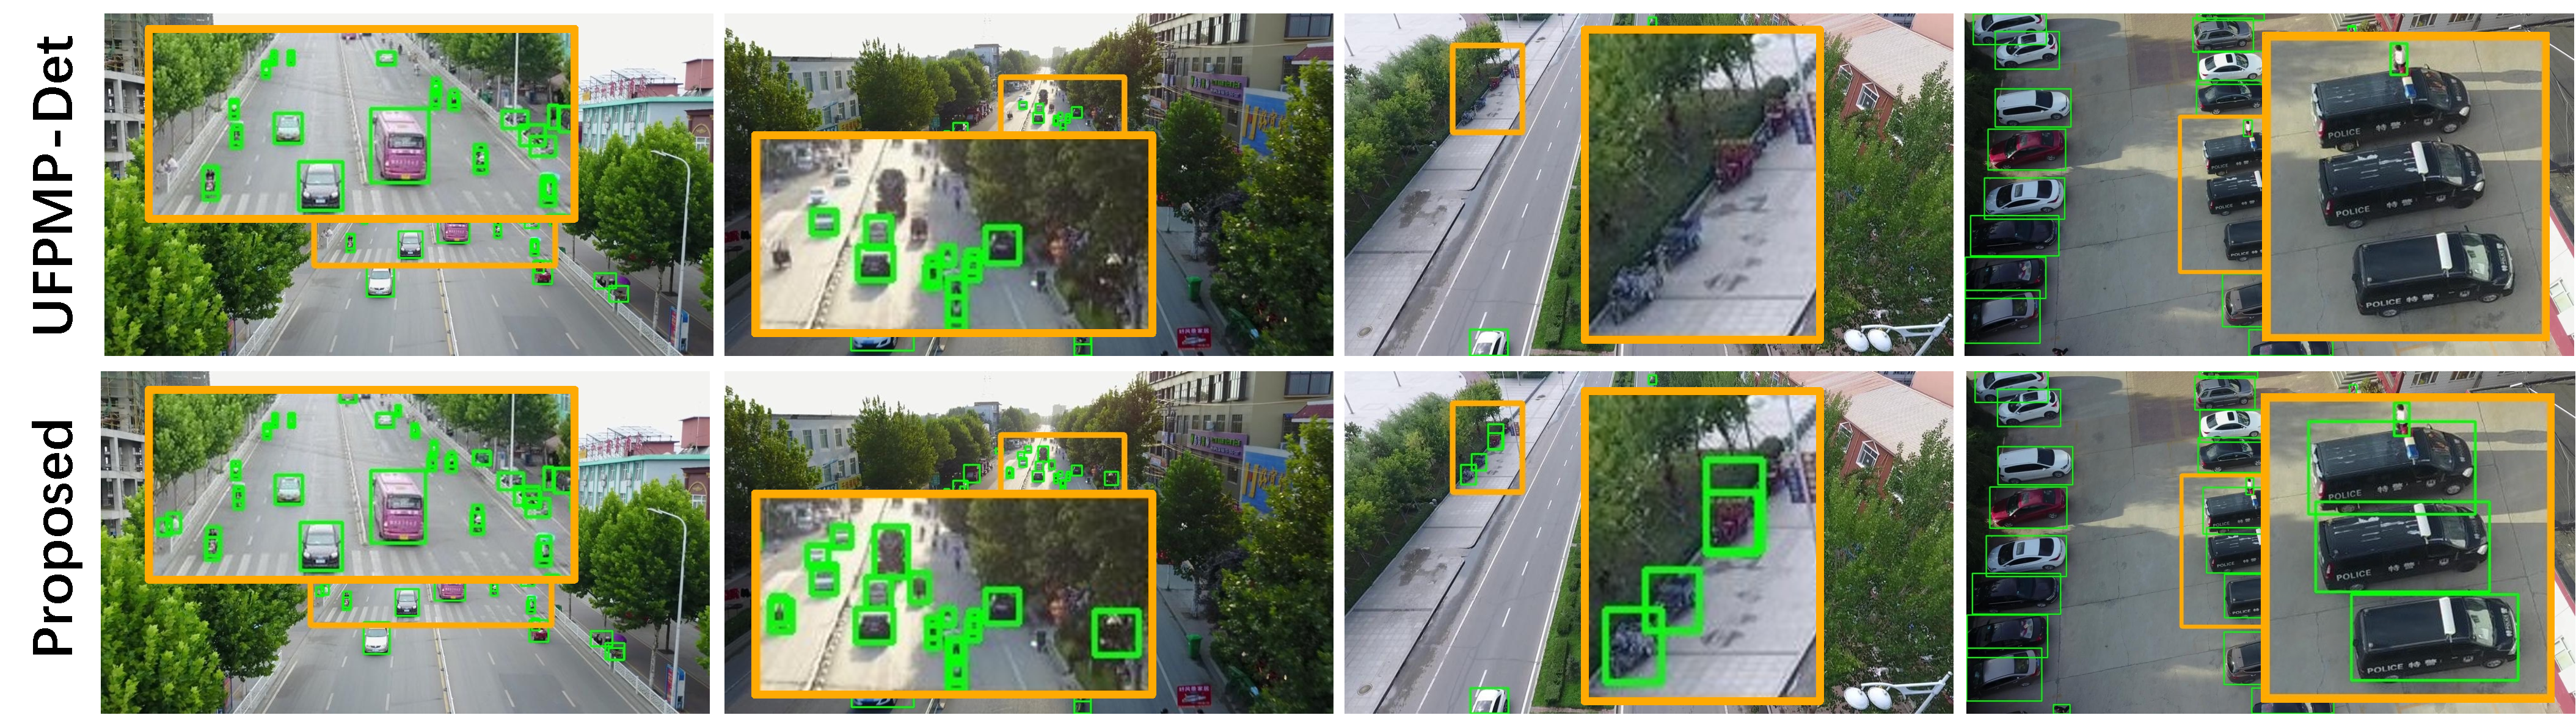
\includegraphics[width=1\linewidth]{images/visualization11.pdf}
	 \caption{Visual comparison with UFPMP-Det~\cite{Huang_2022_UFPMP} on the VisDrone dataset. %Obviously, the proposed method surpasses the compared method with small objects perform.
 % \blue{Objects that are correctly detected are annotated with green bounding boxes. It is obvious that the proposed method can better detect objects, especially ultra-small ones, and handle the large scale variations problem with an adaptive determined optimal scale instead of a fixed scale, while the compared UFPMP-Det cannot.}
 %\rjf{1. Label the method directly on the figure, e.g., replace (a) by UFPMP-Det, (b) by 'Proposed Method'. 2. Discuss w.r.t. the results. E.g. For Image 1 and 2, some discussions. For Image 3 and 4, some discussions. }
 %Focused regions are framed in orange and 
 The proposed method correctly detects more objects than UFPMP-Det, as annotated in green. %\red{More examples can be found in Supplementary Materials.}
 % As shown in the first three columns, the proposed method accurately detects the distant ultra-small objects and well handles the large scale variations, while UFPMP-Det~\cite{Huang_2022_UFPMP} can't. This shows the scale adaptability of our method in detecting objects of different sizes in aerial images. 
 % In the last column, UFPMP-Det wrongly classifies `van' as `car' but the proposed method correctly classifies them, thanks to the exploitation of discriminative information from nearby objects through the spatial semantic attention and the scale consistency. % to exploit the discriminative information from nearby objects. %enhance the difference between inter-class features.}
 }
 \label{fig: visualization}
\end{figure*}

\subsection{Comparison Results on VisDrone}
\label{sssec:visdrone}
% The proposed method is compared with nine state-of-the-art methods on the VisDrone dataset~\cite{Zhu_2022_VisDrone} and the UAVDT dataset~\cite{Du_2018_UAVDT}. 
\begin{table}[!t]
 \centering
 \resizebox{\columnwidth}{!}{
  \begin{tabular}{lccc}
  \hline
  Method & ${AP}$ & ${AP_{50}}$ & ${AP_{75}}$ \\
  \hline
  Faster R-CNN (TPAMI, 2017) & 21.8 & 41.8 & 20.1 \\
  SAIC-FPN (Neurocomputing, 2019) & 35.7 & 62.3 & 35.1 \\
  ClusDet (ICCV, 2019) & 32.4 & 56.2 & 31.6 \\
  % $\text{DMNet}_\text{CVPR Workshop}$~\cite{Li_2020_Density_Workshops} & 29.4 & 49.3 & 30.6 \\
  DMNet (CVPR Workshop, 2020) & 29.4 & 49.3 & 30.6 \\
  GLSAN (TIP, 2021) & 32.5 & 55.8 & 33.0 \\
  HRDNet (ICME, 2021) & 35.5 & 62.0 & 35.1 \\
  Zoom\&Reasoning Det (SPL, 2022) & 39.0 & 66.5 & 39.7 \\
  % \hline
  UFPMP-Det (AAAI, 2022) & 39.2 & 65.3 & 40.2 \\
  % \hline
  UFPMP-Det+MS (AAAI, 2022) & 40.1 & 66.8 & 41.3 \\
  % \hline
  AdaZoom (TMM, 2022) & 40.3 & \textbf{66.9} & 41.8 \\
  \hline
  \multicolumn{1}{l}{Proposed Method} & \textbf{42.2} & 66.0 & \textbf{44.5} \\
  \hline
  \end{tabular}%
  }%
 \caption{Comparisons with state-of-the-art methods on the VisDrone dataset. The proposed method significantly outperforms the compared methods in terms of $AP$ and $AP_{75}$.
 }
 \label{tab:results_visdrone}%
\end{table}%

The comparison results with nine state-of-the-art methods on the VisDrone dataset~\cite{Zhu_2022_VisDrone} are summarized in Table~\ref{tab:results_visdrone}. %We can observe the following from Table~\ref{tab:results_visdrone}. 
Key observations are summarized as follows: 
1)~The proposed model significantly outperforms %all the compared
all compared models in terms of the key evaluation metric $AP$. Specifically, %the proposed method 
it achieves an $AP$ of 42.2\%, making an improvement of 1.9\% over the %previous best performing model
previous best model, AdaZoom~\cite{Xu_2022_AdaZoom}. AdaZoom resizes the patches to a fixed scale, while the proposed method %makes use of 
utilizes the current image patch, the spatial-semantic attention, the scale consistency, and the past experience embedded in the agent to adaptively determine the most appropriate scale for each patch, %and hence achieves 
leading to better detection performance. 2) %The performance gain on $AP_{75}$ is most significant, \eg, compared with the second-best method, AdaZoom, the performance gain is 2.7\%, thanks to the designed Localization Reward, which helps the detector to locate the objects more accurately. 
The most significant performance gain is observed in $AP_{75}$, with a 2.7\% improvement over AdaZoom, thanks to the Localization Reward that enhances object localization. 
3) The proposed method yields a slightly lower $AP_{50}$ than AdaZoom, because many ultra-small objects in the VisDrone dataset only contain a few pixels, while YOLOX faces challenges in detecting these objects during coarse detection~\cite{wang2023improved}. 4) Note that %previous best performing methods 
the previous best methods on the two datasets are different. Compared to the previous best method on the VisDrone dataset, AdaZoom, the proposed method achieves significant performance gains of 7.9\%, 9.3\%, and 10.0\% in terms of $AP$, $AP_{50}$ and $AP_{75}$, respectively, on the UAVDT dataset.

\subsection{Ablation Study of Major Components}
\label{ssec: ablation-study}
The ablation results for the proposed method on the VisDrone dataset~\cite{Zhu_2022_VisDrone} are summarized in Table~\ref{tab:ablation}.
% 1) Compred with
1) Compared to the YOLOX baseline, by introducing the PPO agent to determine the optimal scales based on the appearance feature extracted directly from the Patch Encoder, the $AP$, $AP_{50}$ and $AP_{75}$ are improved by 1.6\%, 2.6\% and 1.8\%, respectively. 
2) By adding the spatial-semantic attention (SSA) into the visual perception module, the $AP$, $AP_{50}$ and $AP_{75}$ are further improved by 1.6\%, 2.1\% and 1.9\%, respectively. 
%2) \blue{Adding spatial-semantic attention (SSA) to the visual perception module further enhances $AP$, $AP_{50}$, and $AP_{75}$ by 1.6\%, 2.1\% and 1.9\%, respectively.}
3) By incorporating the evolutionary strategy into the PPO agent, the $AP$, $AP_{50}$ and $AP_{75}$ are further boosted by 1.5\%, 2.0\% and 1.5\%, respectively. 
%3) \blue{Incorporating the evolutionary strategy into the PPO agent boosts $AP$, $AP_{50}$, and $AP_{75}$ by 1.5\%, 2.0\% and 1.5\%, respectively.}
The proposed EVORL makes good use of the past experience to refine the derived scaling factors, so that it mitigates the outlier scaling factors. These ablation results show the effectiveness of the major components in the proposed method. 
%\blue{makes good use of past experience to refine scaling factors, reducing the impact of outlier factors. These ablation results show the effectiveness of the major components.}  

\begin{table}[!t]
 \centering
  \begin{tabular}{cccccccc}
  \hline
  YOLOX & PPO & SSA & EVO & ${AP}$ & ${AP_{50}}$ & ${AP_{75}}$ \\
  \hline
  $\surd$ & & & & 37.5 & 59.3 & 39.3 \\
  $\surd$ & $\surd$ & & & 39.1 & 61.9 & 41.1 \\
  $\surd$ & $\surd$ & $\surd$ & & 40.7 & 64.0 & 43.0 \\
  $\surd$ & $\surd$ & $\surd$ & $\surd$ & \textbf{42.2} & \textbf{66.0} & \textbf{44.5} \\
  \hline
  \end{tabular}%
 \caption{Ablation study of major components of the proposed method on the VisDrone dataset. 
 }
 \label{tab:ablation}%
\end{table}%
% consistently improves the detection performance of baseline models that directly detect objects on drone-captured images. These results show the importance of determination of the optimal scale for dealing with small object detection, verify the effectiveness of the proposed constraint and RL in handling the missing label problem , and reflect the effectiveness of the designed object-attentional mechanism to exploit the spatial semantic relations between objects. Moreover, the comparison results of the last two combinations illustrate the benefits of introducing the evolutionary strategy into the model to address the unlabel problem, i.e., the determination of optimal scale for each generated clustered regions.}


% \subsubsection{Analysis of Proposed Model Structure} 
% \label{sec: ablation-modules} 
% An ablation study is carried out to evaluate the proposed small scale feature map strategy and the reinforcement learning based adaptive scale ratio selection algorithm. Results are demonstrated in Table~\ref{tab:ablation_structure} where SSFM and RLAS represent the `small scale feature map' and `RL adaptive scale' module, respectively. 
% %The compared methods are summarized as follows.



\subsection{Visualization of Detection Results}
\label{ssec:visualization}
The proposed method is visually compared %with 
to UFPMP-Det~\cite{Huang_2022_UFPMP} that yields the previous best results averaged across the two datasets. As shown in Fig.~\ref{fig: visualization}, the proposed model better recognizes small objects that are easily neglected, \eg, the `car' and `person' objects at the lower left corner of the focused regions in the first two columns, and the `tricycle' objects in the third column. The ultra-small feature map encodes more low-level but high-resolution features, partially reducing the %issue of losing 
loss of details during feature pooling. %More importantly UFPMP-Det selects one of the three predefined scaling factors by considering the average object size in a patch only
Notably, UFPMP-Det selects one of three predefined scaling factors based on the average object size in a patch, while the proposed method adaptively determines the optimal scale of each patch by utilizing both the current patch and %the past experience embedded in the agent. 
the agent's past experience, and hence better detects small objects. Moreover, as seen from the last column of Fig.~\ref{fig: visualization}, UFPMP-Det wrongly classifies 
`van' as `car' whereas the proposed method can correctly classify them, thanks to the proposed scale-consistency reward and the spatial-semantic attention mechanism, which %make good use of the supportive information from nearby objects to better distinguish these challenging objects. 
effectively utilizes supportive information from nearby objects to better distinguish challenging objects. 

\section{Conclusion}
\label{sec: conclusion}
To tackle the challenges of detecting small objects and handle the large scale variations in drone imagery, an evolutionary reinforcement learning framework %is
has been proposed to determine the optimal scale for object detection. %each patch, at which the object could be more precisely detected following a coarse-to-fine strategy. %The proposed model follows a coarse-to-fine strategy and aims to determine the optimal scale for each coarse generated region, which is a critical but often overlooked factor in preceding aerial object detection solutions.
The designed agent combines the evolutionary strategy and the proximal policy optimization strategy to make good use of both the current patch status and the past experience embedded in the agent's population. The three designed rewards, considering the localization accuracy, the accuracy of predicted labels, and the scale consistency, address the issue of lacking ground-truth labels for optimal scales, and provide supervision signals for training the agent. Furthermore, a spatial-semantic attention %is
has been designed to capture the mutual supportive information from nearby objects. The proposed method %is 
has been compared with nine state-of-the-art approaches on two benchmark datasets, UAVDT and VisDrone. It significantly outperforms the compared solutions. %, achieving state-of-the-art object detection accuracy. 


\section{Acknowledgement}
This work was supported in part by the National Natural Science Foundation of China under Grant 72071116, and in part by the Ningbo Municipal Bureau of Science and Technology under Grant 2019B10026, 2021Z089 and 2022Z173.

% \newpage
\bibliography{aaai24}

\end{document}